\documentclass[12pt, a4paper]{report}

\setlength{\parindent}{0pt}
% Packages
\usepackage{amsmath}
\usepackage{bm}
\usepackage{subcaption}
\usepackage{cancel}
\usepackage{subcaption}
\usepackage[utf8]{inputenc}   % Allows the use of UTF-8 encoded characters
\usepackage[dvipsnames]{xcolor} % add more colors
\usepackage{amsmath, amssymb} % Provides advanced mathematical tools and symbols
\usepackage{amsthm}           % Allows the creation of theorem-like environments
\usepackage{cancel}
\usepackage{colortbl} % For coloring cells
\usepackage{tcolorbox} % For coloring cells with smaller background
\usepackage{tikz} % For dags
\usepackage{graphicx}
\usepackage{subcaption}
\usepackage{algorithm}        % Provides an environment for writing algorithms
\usepackage{algpseudocode}    % Used in conjunction with 'algorithm' for algorithmic pseudocode
\usepackage{graphicx}         % Allows for the inclusion of graphics (images)
\usepackage[]{xcolor}         % Provides tools for color management in documents
\usepackage{hyperref}         % Enables hyperlinks within the document
\usepackage{caption}          % Customizes the appearance of captions for figures and tables
\usepackage{float}            % Improves the placement of figures and tables
\usepackage{geometry}         % Allows for the customization of page layout and margins
\usepackage{setspace}         % Enables control over line spacing
\usepackage{times}            % Uses Times New Roman font
\usepackage{titlesec}         % Provides tools for customizing section titles
\usepackage[backend=biber, style=numeric, sorting=ynt]{biblatex} % Manages bibliography with biber backend, numeric style, and sorts entries by year, name, title

% Geometry package for setting margins
\geometry{
  left=2.5cm,
  right=2.5cm,
  top=2.5cm,
  bottom=2.5cm,
}

%--------------------------------------------------------------------------

\titleformat{\chapter}[display]
  {\normalfont\LARGE\bfseries}{\chaptertitlename\ \thechapter}{20pt}{\Huge}
\titleformat{\section}
{\normalfont\Large\bfseries}
{\thesection}{1em}{}
\titleformat{\subsection}
{\normalfont\Large\bfseries}
{\thesubsection}{1em}{}
\titleformat{\subsubsection}
{\normalfont\large\bfseries}
{\thesubsubsection}{1em}{}
\DeclareCaptionFont{}{}
\captionsetup{labelfont={bf}}
\renewcommand{\arraystretch}{1.4} % Enlarge cells in tables

\newcommand{\RNum}[1]{\uppercase\expandafter{\romannumeral #1\relax}}

\addbibresource{ref.bib}

% Line spacing
\onehalfspacing

\theoremstyle{definition}
\newtheorem{definition}{Definition}[chapter]

\theoremstyle{plain}
\newtheorem{theorem}{Theorem}[chapter]
\newtheorem{lemma}[theorem]{Lemma}

\theoremstyle{remark}
\newtheorem{remark}{Remark}[chapter]

% Custom command to format Introduction
\newcommand{\introchapter}{
  \chapter*{Introduction}
  \addcontentsline{toc}{chapter}{\numberline{1}Introduction}
  \markboth{Introduction}{Introduction}
  \setcounter{chapter}{0}
}

% Custom command to format Conclusion
\newcommand{\conclchapter}{
  \chapter*{Conclusion}
  \addcontentsline{toc}{chapter}{\numberline{6}Conclusion}
  \markboth{Conclusion}{Conclusion}
  \setcounter{chapter}{6}
}

% Independence command
\newcommand{\independent}{\protect\mathpalette{\protect\independenT}{\perp}}
\def\independenT#1#2{\mathrel{\rlap{$#1#2$}\mkern2mu{#1#2}}}

%dependence command
\newcommand{\dep}{\not\!\perp\!\!\!\perp}

% Backslash command
\newcommand{\textbackslash}{\texttt{\symbol{92}}}

% Title Page
\begin{document}
\title{THESIS TITLE}
\author{Jacopo Palombarini}
\date{2024}

%----------------------------- Frontispiece
\pagenumbering{gobble} % Suppress page numbers for the title page and other preliminary pages
\newgeometry{margin=0.8in}
\begin{titlepage}
    \begin{center}
        \vspace*{0.2cm}
        {\fontsize{19pt}{20pt}\selectfont \textbf{Alma Mater Studiorum - Università di Bologna}\par}
    
        \noindent\hrulefill
        \vspace{0.8cm}
        
        \Large
        
        Department of Statistical Science \\
        Second Cycle Degree in Statistical Sciences
        
        
        
        \Large
        \vspace{5cm}
        {\fontsize{22.5pt}{22.5}{\textbf{Causal Inference in Multivariate Time Series: a Machine Learning-based prospective}}}

        
     
        \vspace{4.5cm}
         \begin{minipage}[t]{0.48\textwidth}
        \begin{flushleft}
            {\fontsize{16pt}{16pt}\textbf{Presented by:} \\ Jacopo Palombarini \\ 0001076600}
        \end{flushleft}
    \end{minipage} 
    \begin{minipage}[t]{0.48\textwidth}
        \begin{flushright}
            {\fontsize{16pt}{16pt}\textbf{UNIBO Supervisor:} \\ Prof. Pietro Rigo\\
            {\fontsize{16pt}{16pt}\textbf{ULB Supervisors:} \\ 
            Prof. Gianluca Bontempi\\
            Prof. Gian Marco Paldino}
        \end{flushright}
    \end{minipage}
        
        
        \vfill
        \noindent\hrulefill
        \vspace{0.3cm}
        \Large
        
       
        
        \RNum{2} SESSION \\
        Academic Year 2023/2024
    \end{center}
\end{titlepage}
\restoregeometry
\vspace*{5cm}
\begin{flushright}
  {\parbox{4.2cm}{\textit{}}}
\end{flushright}
% ----------------------------------------------

% ----------------------------- Abstract
\clearpage
\pagenumbering{roman} % Start Roman numerals from the abstract
\begin{abstract}
\noindent
An abstract typically under 200 words should summarize the core parts of the thesis. Specifically, the abstract should include the motivation for the study, statement of the research problem, the methodology used and the results and conclusions of the study.\\
\textbf{Keywords:} keyword1, keyword2, keyword3, keyword4, keyword5
\end{abstract}

% ----------------------------- Table of Contents
\tableofcontents
\clearpage

% ----------------------------- Main Content
% Introduction
\introchapter
\pagenumbering{arabic} % Switch to Arabic numerals for the main content
\input{chapters/2 Introduction.tex}

\chapter{Theoretical Background}\label{Theoretical Background}
This first chapter wants to give an overview of all the theoretical concepts behind the methods that are applied in the second part of the thesis.
We are going to see what a time series is and what are the main statistical tools to analyze time series from a causal point of view.


% Sections:
% 1 Causal Inference for Time Series
% 2 State-of-the-art Methods
% 3 D2C, caD2C and TD2C
\section{Causality, Causal Inference \& Causal Discovery}
In this section we are going to define Causality and its derivations in mathematical and statistical fields.\\

We can define causality as the consequential relationship between two objects, a cause and an effect. A causal relationship underlines a connection, between two or more events, imposing a directionality, so that one of those events occurs, time-wise, before the others, and it can't be the other way around. J.Pearl - one of the greatest contributors in the causality field - proposed this simple definition: \textit{A causes B if B listens to A} (The Book of Why, Pearl \& Mackenzie, 2019). \\

Causality goes beyond the concept of correlation - \textit{correlation is not causation} - which only requires that two variables are connected and show dependency, but without imposing an order between them, i.e., one variable is not a consequence of the other, but just connected to it.\\
For the same reasons that discovering, analyzing and predicting the associations between variables is so important, knowing that we can (directly or indirectly) influence some aspects of the world we observe by controlling some of its features, is also quite attractive.
Aristotle, one of the most important philosophers of ancient Greece, believed that comprehending the causal structure of a process is a crucial element in understanding this process. (\cite{molak2023causal}). To cite another important philosopher, David Hume contended that causation relies on experience, which means any perceived cause-and-effect relationship could be erroneous. He maintained that since thoughts are subjective, it is impossible to definitively establish causality. Despite this quite skeptical interpretation of causality, we can still find, in statistical literature, some methods and techniques that aim to find strong enough evidences of consequential connections between events. From 1920 - when Sewall Wright, for the first time, put down mathematically the assumption that X causes Y and not the other way around (\ref{fig0}) (\cite{pearl2022causal}) - researchers started to develop an interest in what we today call Causal Learning. \\

\begin{figure}
    \centering
    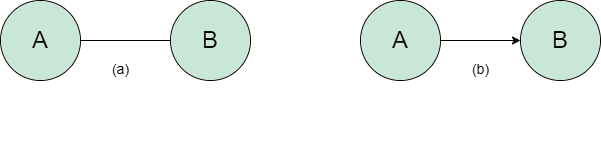
\includegraphics[width=0.8\linewidth]{chapters/Images/Causality_vs_dependency.png}
    \caption{Dependency relation (a) and causality relation (b)}
    \label{fig0}
\end{figure}

Causal Learning encompasses two primary processes, both rely on observational or interventional data. The first, Causal Inference (Ci), aims to quantify the impact of a cause on its effect and relies heavily on a formal representation of the interactions among observed variables, called a causal graph. Despite its simplicity, this graphical representation is very effective for enhancing explainability. When the causal graph is unknown, it is possible to identify cause-effect pairs by integrating available data with prior knowledge. The second process, known as Causal Discovery (CD), aims to derive those causal connections within the system, it's a set of methods meant to recover the structure of the data-generating process from the data generated by that process. Recently, Causal Discovery has seen significant advancements, and this progress has led to the fragmentation of the field into various subfields, each with different assumptions, problems, and solutions, although they share the same ultimate goal (\cite{zanga2022survey}). Causal discovery methods and their application are at the core of this study and some of them are going to be deepened in section \ref{State-of-the-art Methods}.\\

\subsection{Simpson paradox and other examples and images to make causation more clear}
Here we display some examples to clarify the essential concept of causality, which may not be easily comprehended by someone who is used to thinking solely in terms of statistical correlation.
Let's start with one of the most famous effects of causation: the Simpson's paradox.
The paradox refers to the existence of data in which a statistical association that holds for an entire population is reversed in every subpopulation (i.e. considering subpupulations of data marked by a specifica variable's categories). This effect can help us a lot in understanding the logic behind causation because it shows us how a simple association between two variables can be denied and changed by considering a third variable that influences both the other two. 
Let's take, for example, three variables from a passed investigation about female smokers, their age, their smoker status (positive or negative) and their survival after 20 years from the first data collection (positive or negative). The marginal contingency table is here displayed:

\begin{table}[!ht]
    \centering
    \caption{Marginal table between the variables \textit{Smoker} and \textit{Survival state}. In green, the smallest survival rate between the two.}
    \begin{tabular}{r|ll}
        \textbf{} & \textbf{Alive} & \textbf{} \\ \hline
        \textbf{Smoker} & yes & no \\ \hline
        yes & 76,1\% & 23,9\% \\ 
        no & \color{Green}68,6\% & 31,4\% \\ 
    \end{tabular}
    \label{sp1}
\end{table}

As we notice in Table \ref{sp1}, smoking seems to favour the survival of considered subjects. In contrast, if we consider percentages in the partial contingency Table \ref{sp2} we see how this trend is reversed by including the third variable, \textit{Age}, and conditioning on it, i.e. by sorting data using its categories (1 = "Age $\leq 24$", 2 = "$24 <$ Age $\leq 65$", 3 = "Age $> 65$").

\begin{table}[!ht]
    \centering
    \caption{Partial contingency table, both in frequencies and percentages,  between the variables \textit{Smoker} and \textit{Survival state}, grouped by variable \textit{Age}. In green, the smallest survival rate per age category.}
    \begin{tabular}{r|ll|ll|ll}
        \multicolumn{7}{c}{\textbf{Percentages}} \\
        Age &  1 & ~ & 2 & ~ & 3 & ~ \\ \hline
        Smoker / Alive & yes & no & yes & no & yes & no \\ \hline
        yes & \color{Green}96.4\% & 3.6\% & \color{Green}80.3\% & 19.7\% & \color{Green}12.2\% & 87.8\% \\
        no & 98.6\% & 1.4\% & 84.5\% & 15.4\% & 13.9\% & 86.1\% \\
    \end{tabular}
    
    \vspace{1cm}
    
    \begin{tabular}{r|ll|ll|ll}
        \multicolumn{7}{c}{\textbf{Frequencies}} \\
        Age &  1 & ~ & 2 & ~ & 3 & ~ \\ \hline
        Smoker / Alive & yes & no & yes & no & yes & no \\ \hline
        yes & 53 & 2 & 384 & 94 & 6 & 43 \\
        no & 71 & 1 & 406 & 74 & 25 & 155 \\
    \end{tabular}
    \label{sp2}
\end{table}


Here, it's clear how smoking has a negative impact on survival rate in every age category. This is possible because, as we see also in \ref{fig6}, the variable \textit{Age} causes both the other two variables, and this changes their relation. This back-and-forth consideration of more variables can continue indefinitely, revealing a persistent challenge. Simple statistics cannot resolve this issue, as no statistical method alone can uncover the true causal relationships within the data. To determine the actual causal connections among the variables, we must first comprehend the underlying story and mechanisms that produced the observed results. Statisticians often interpret data with strong causal assumptions. In such cases, the paradox would disappear because the causal story could align with our example’s structure. However, even though the assumption that "smoking does not cause age" might seem obvious, it cannot be tested within the data itself. Moreover, causal information cannot be represented in contingency tables, which are frequently used for statistical inference. (\cite{pearl2016causal})\\

\textbf{\textit{Other examples}}\\

\subsection{Causality framework exploration}\label{Causality framework exploration}
Before proceeding, we would like to clarify, as completely as possible, all the statistical purposes bounded with the concept of causality. These purposes are in constant evolution, but we think it could be useful to portray the current state of this field to better understand the intents and the positioning in the literature of all the following topics.\\

As previously mentioned, causality learning objectives can be divided into two categories: determining causal effects, referred to as Causal Inference or Parameter Learning, and identifying causal relationships between objects, known as Causal Discovery or Structural Learning. Although these two areas intersect to some extent, their definitions differ slightly.
Understanding the causal relationships among variables typically involves determining the correct causal directions, causal lags, and associated causal indices. In contrast, learning about causal effects focuses on infer the impact of altering one variable on the outcome of another, given that some variables are already known to have causal connections.(\cite{chang2021multivariate})\\

These two purposes branch out, following various criteria, in different approaches. While studying causality and its application, the amount of methods in the literature could get confusing, that's why we provide, in Figure \ref{fig:1}, a concise summary of them in a schematic way.  

\begin{figure}[!h]
    \centering
    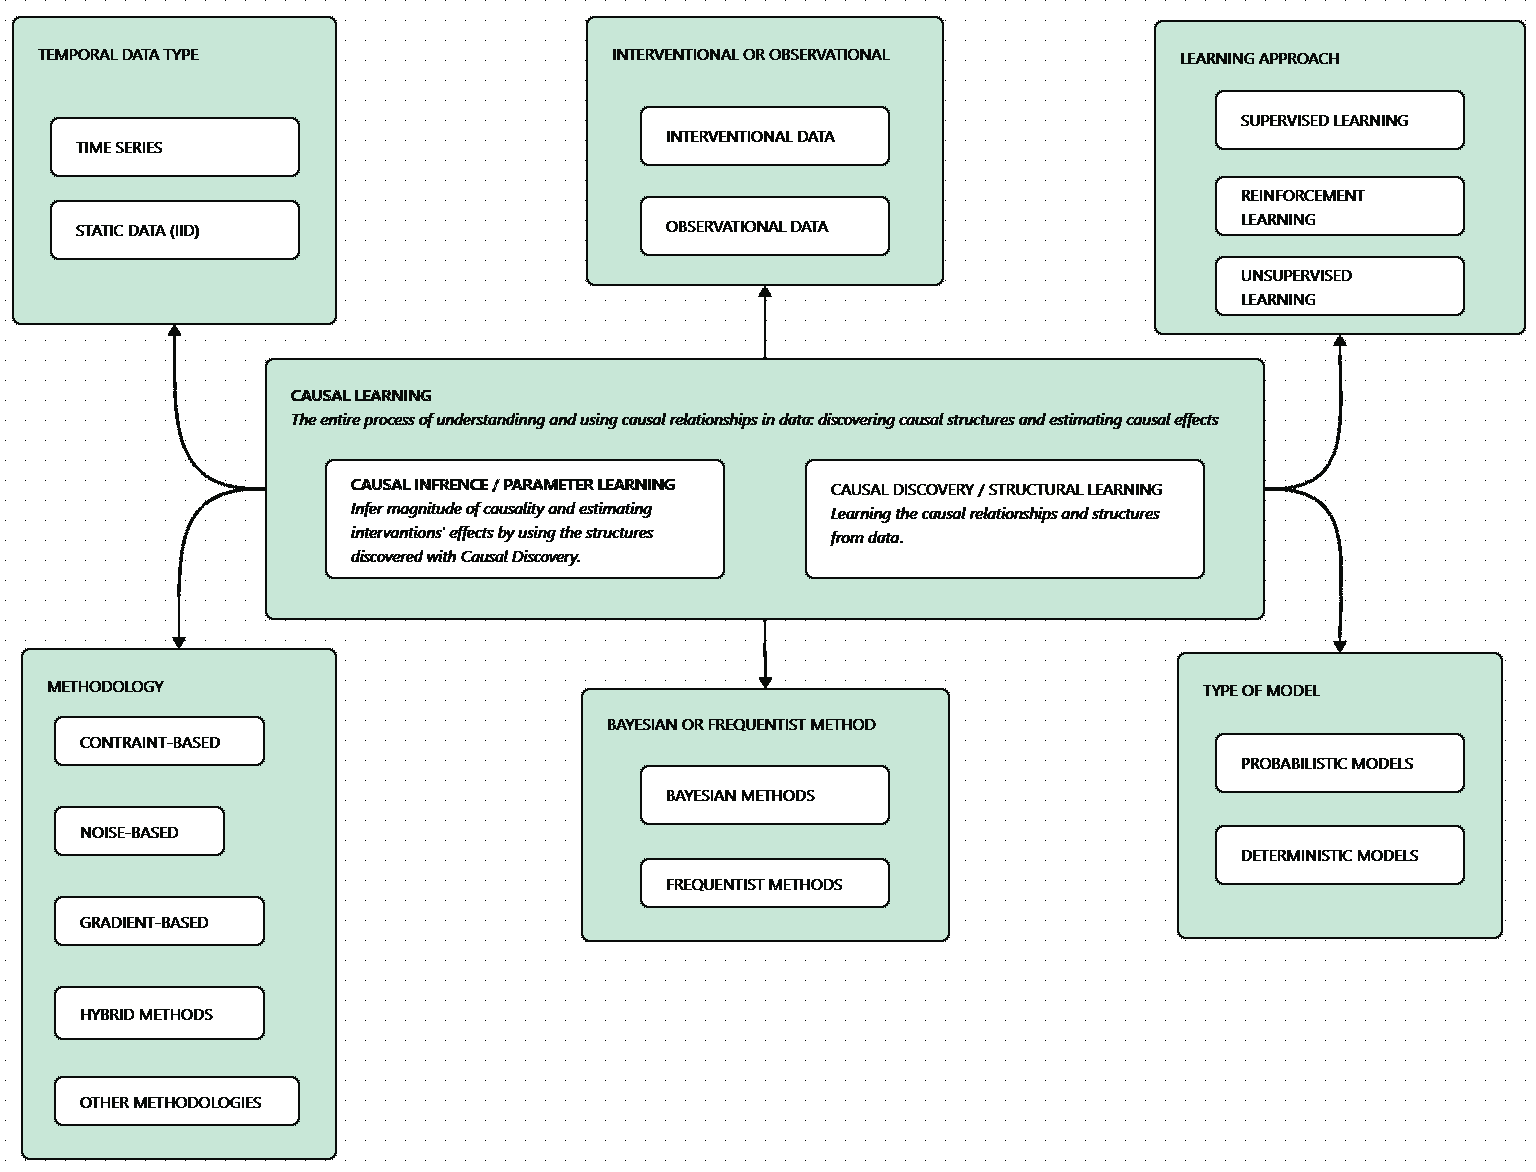
\includegraphics[width=1\linewidth]{chapters//Images/Causal Learning scheme.png}
    \caption{Ways of categorizing methods and approaches in Causal Learning context. In blue, we underlined TD2C's characteristic}
    \label{fig:1}
\end{figure}

\section{Fundamental tools}
This quite technical section is going to give us some important definitions that revolve around the Causality world. We dedicate this section of the thesis to theoretical concepts that require some specifications and that will be mentioned in the subsequent parts, or that are just useful to have a wider comprehension of the context.\\

We start with the definition of some fundamental concepts about causal relationships and causal effects.\\

\begin{definition}[Conditional Probability]
    Conditional Probability is the probability of one event, given that another event has occurred. $P(X|Y),$ where "$|$" stays for "given that".
\end{definition}
The complete notation is $P(X = x|Y = y)$: "the probability that the variable X takes the value x, given that the variable Y takes the value y". It can be also adapted to continuous cases, where we refer to probability densities.
\begin{definition}[Confounding]
    A confounding variable influences two or more other variables and produces a spurious association between them. From a purely statistical point of view, such associations are indistinguishable from the ones produced by a causal mechanism (\ref{fig6}).
\end{definition}

\begin{figure}[!h]
    \centering
    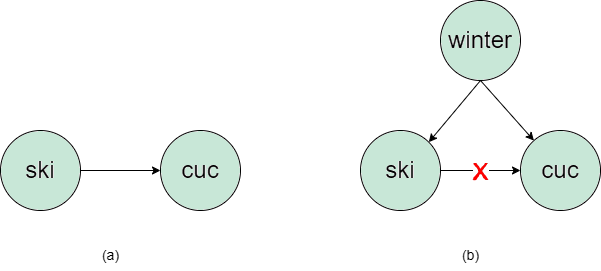
\includegraphics[width=0.7\linewidth]{chapters/Images/confounding.drawio.png}
    \caption{Example of confounding: from a first look (a) the increase in people going skiing at a certain time causes the decrease in sales of cucumbers, but, including the \textit{confounder} "winter season" (b), we are able to remove the causality between the previous two variables, since the new one causes them both.}
    \label{fig6}
\end{figure}

A very important aspect of a properly designed randomized experiment (RCT) is that it allows us to avoid confounding.
\begin{definition}[Intervention]\label{int}
     Intervention is changing one thing in the world and the observing whether and how this change affects another thing in the world.
\end{definition}

Interventions are the essence of scientific experiments. To describe interventions mathematically, we use the do-operator \ref{doo}: $P(Y = 1 | do(X = 0)$. While conditioning only modifies our view of the data, interventions affects the distribution by actively setting one (or more) variable(s) to a fixed value or distribution. \cite{molak2023causal}

\begin{definition}[Counterfactual]\label{count}
    Counterfactuals are estimates of how the world would look if we changed the value of one or more variables, holding everything else constant.
\end{definition}

Because, we can never observe the same event under two mutually exclusive conditions at the same time, counterfactuals cannot be observed, and so the true causal effect is always unknown. Two different counterfactual causal models can lead to the same interventional distribution.\\

Interventions and Counterfactuals, togheter with Associations, are the three steps of the so-called \textit{Ladder of Causation} described by Judea Pearl.
Each step answers to different causal questions:  association is related to observing, using association, we can answer questions about how seeing one thing changes our beliefs about another thing;  the action related to step two is doing (\ref{int}); activities associated with step three are imagining and understanding (\ref{count}).\\


\begin{definition}[do-operator]\label{doo}
    
\end{definition}

\textit{\textbf{Little digression on do-calcolus (Molak's book)}}\\

Then, we need some definitions about DAGs and SCMs.\\

\begin{definition}[Graph]
    A graph $G = (V, E)$ is a mathematical object represented by a tuple of two sets: a finite set of vertices $V$ and a finite set of edges $E \subseteq VV$. If not specified otherwise, this graph is intended as an undirected graph, where the undirected edge $(X, Y)$ is identical to the edge $(Y, X)$ and its graphical representation is $X - Y$.
\end{definition}

\begin{definition}[Directed Graph]
    A directed graph (DG) is a graph where the edge $(X, Y)$ is distinct from the edge $(Y, X)$.
\end{definition}
In particular, a directed edge $(X, Y)$ is graphically represented by an arrow as $X \rightarrow Y$, and induces a set of relationships between the vertices of the graph $G$. Given a vertex $X$, we denote by $Pa(X)$ its parents, i.e. the set of vertices that have an arrow into $X$, while we denote by $Ch(X)$ its children, i.e. the set of vertices that have an arrow out of $X$. Recursively, any parent and parent of a parent (child and child of a child) of $X$ is an ancestor $An(X)$ (descendant $De(X)$) of $X$.
The vertices connected to $X$ are said to be adjacent to $X$ and denoted by $Adj(X)$, while the vertices connected with an undirected edge are the neighbors $Ne(X)$. These two sets of vertices are identical in undirected graphs, but may be different in graphs with other mixed orientations.
\begin{definition}[Adjacency matrix]
    Adjacency matrices are square $M$ × $M$ matrices where $M$ is the number of nodes. Each positive entry in the matrix encodes an edge between a pair of nodes (\ref{fig7}).
\end{definition}

\begin{figure}[h!]
    \centering
    \begin{subfigure}[b]{0.45\textwidth}
        \centering
        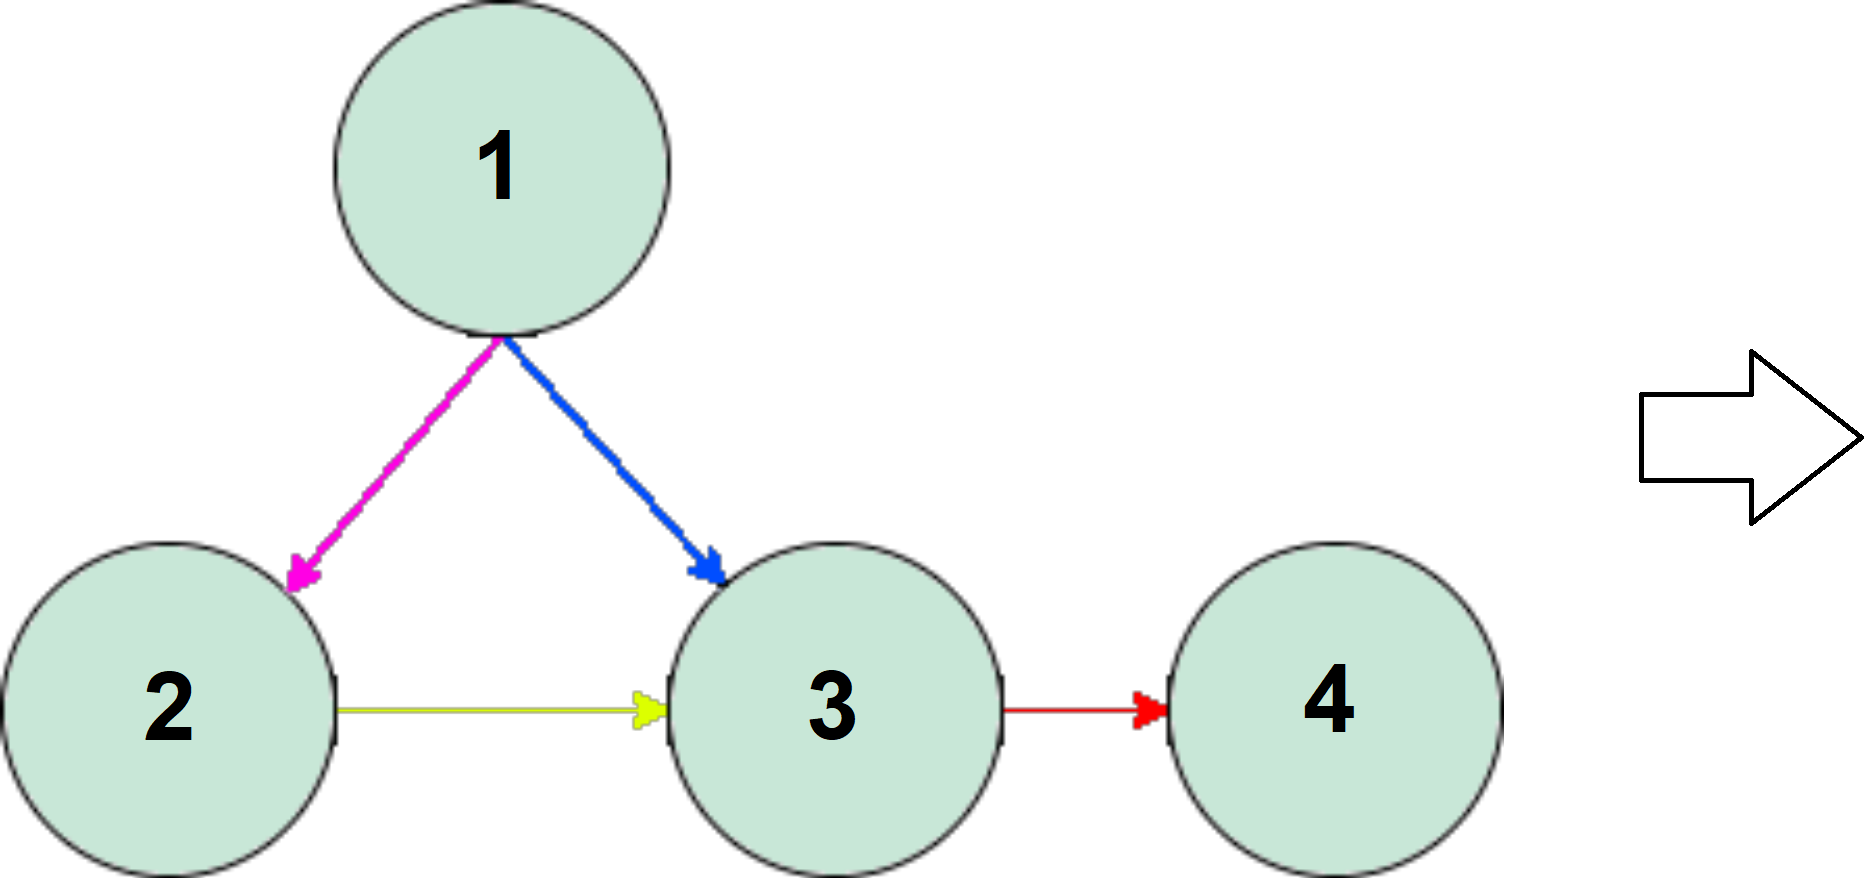
\includegraphics[width=1.2\linewidth]{chapters/Images/DAG.png}
        \caption{}
        \label{fig:dag}
    \end{subfigure}
    \hfill
    \begin{subfigure}[b]{0.5\textwidth}
        \centering
        
        \[
        \renewcommand{\arraystretch}{2}
        \setlength{\arraycolsep}{1.5em}
        \begin{bmatrix}
        0 & \tcbox[colback=RubineRed, boxrule=0pt, arc=0pt, left=1pt, right=1pt, top=1pt, bottom=1pt]{1} & \tcbox[colback=NavyBlue, boxrule=0pt, arc=0pt, left=1pt, right=1pt, top=1pt, bottom=1pt]{1} & 0 \\
        0 & 0 & \tcbox[colback=Yellow, boxrule=0pt, arc=0pt, left=1pt, right=1pt, top=1pt, bottom=1pt]{1} & 0 \\
        0 & 0 & 0 & \tcbox[colback=Red, boxrule=0pt, arc=0pt, left=1pt, right=1pt, top=1pt, bottom=1pt]{1} \\
        0 & 0 & 0 & 0 \\
        \end{bmatrix}
        \]
        \caption{}
        \label{fig:adjacency-matrix}
    \end{subfigure}
    \caption{A Directed Acyclic Graph (a) and its Adjacency Matrix (b).}
    \label{fig7}
\end{figure}

\begin{definition}[Path (Directed path)]
    A path (Directed path) $\pi = (X - ... - Y)$ ($\pi = (X \rightarrow ... \rightarrow Y)$) is a tuple of non repeating vertices, where each vertex is connected to the next in the sequence with an undirected (directed) edge.
\end{definition}
\begin{definition} [Directd Acyclic Graph]: 
    A directed acyclic graph (DAG) is a directed graph G that has no cycles.
\end{definition}
\begin{definition}[Causal Graph]
    A causal graph $G = (V, E)$ is a graphical description of a system in terms of cause-effect relationships, i.e. the causal mechanism.
\end{definition}
\begin{definition}[Causal edge assumption]
    The value assigned to each $X$ is completely determined by the function $f$ given its parents: $X := f (Pa(X)) ∀X ∈ V$.
\end{definition}
\begin{definition}[Structural causal model]
    A structural causal model(SCM) is defined by the tuple $M = (V, U, F, P)$, where:
    \begin{itemize}
        \item $V$ is a set of endogenous variables, i.e. observable variables
        \item $U$ is a set of exogenous variables, i.e. unobservable variables, where $V \cap U = \emptyset$
        \item $F$ is a set of functions, where each function $f \in F$ is defined as $f_i : (V \cup U)^p \rightarrow V$, with $p$ the ariety of $f$, so that $f$ determines completely the value of $V_i$
        \item $P$ is a joint probability distribution over the exogenous variables $P(U) = \prod_i P(U_i)$.
    \end{itemize}
\end{definition}

SCMs consist of a set of exogenous (noise variables, root variables) and endogenous (observable variables) variables and a set of functions defining the relationships between these variables. They can be represented as graphs, with nodes representing variables and directed edges representing functions and they can produce interventional and counterfactual distributions. To represent a SCM we can use a set of equations or a graph, as in figure \ref{scm}.\\

\begin{figure}[!h]
\centering
\begin{tikzpicture}[
  every node/.style={draw, circle, minimum size=1.5cm, font=\large},
  dashed node/.style={draw, circle, dashed, minimum size=1.5cm, font=\large},
  solid edge/.style={draw,->,thick}
]
% Define the nodes
\node[dashed node] (A) at (0,2) {$U_0$};
\node[dashed node] (B) at (3,2) {$U_1$};
\node[dashed node] (C) at (6,2) {$U_2$};
\node (D) at (0,-1) {$X$};
\node (E) at (3,-1) {$Y$};
\node (F) at (6,-1) {$Z$};
% Define the edges
\path[solid edge] (A) edge (D);
\path[solid edge] (B) edge (E);
\path[solid edge] (C) edge (F);
\path[solid edge] (D) edge (E);
\path[solid edge] (E) edge (F);
\end{tikzpicture}
\caption{An example of Structural Causal Model with exogenous (dashed circles) and endogenous (solid circles) variables}
\label{scm}
\end{figure}


\begin{definition}[Causal discovery problem]
    The causal discovery problem consists in recovering the groundtrouth graph $G^*$ (that generated $D$) from the given dataset $D$.
\end{definition}
\begin{definition}[Soundness and completeness of a Causal Discovery algorithm]
    A causal discovery algorithm is sound if it is able to solve the causal discovery problem, and it is complete if it outputs the most informative causal graph $G$ that can be recovered from the input dataset $D$, without making further assumptions.
\end{definition}
\begin{definition}[Markov property]\label{MP}
    A graph $G =(V, E)$ is said to satisfy the Markov property if the associated joint probability distribution $P(V)$ can be decomposed recursively as: $P(V) = \prod_{X \in V} P(X|Pa(X))$
\end{definition}
The probability factorization expressed in Definition \ref{MP} relies on the assumption that the relationships encoded by the graph match exactly the underlying conditional probability independencies:
$X \independent_P Y | Z \Rightarrow X \independent_G Y | Z$ where $Z$ is a subset of $V/{X, Y}$.
Essentially, it is assumed that the probability independence ($\independent_P$) implies the graphical independence ($\independent_G$).
\begin{definition}[Forks, Chains and Colliders]\label{fcc}
     Let $G =(V, E)$ be a DG and $\pi$ be a path on $G$. Then, given three vertices $X$, $Y$ and $Z$ in $\pi$, we have the following:
     \begin{itemize}
         \item $X\leftarrow Y \rightarrow Z$ is a fork on $\pi$
         \item $X \rightarrow Y \rightarrow Z$ is a chain on $\pi$
         \item $X \rightarrow Y \leftarrow Z$ is a collider on $\pi$
     \end{itemize}
\end{definition}

Testing for conditional independence (CI) between the variables is one of the most important techniques
to find the causal relationships among the variables (it is the core of \ref{Constraint-bsed Methods}). Conditional independence between two variables $X$ and
$Y$ results when they are independent of each other given a third variable $Z$ (i.e. $X \independent Y | Z$). In the case of causal discovery, CI testing allows deciding if any two variables are causally connected or disconnected. An important criterion for CI testing is the d-separation criterion which is formally defined in \ref{d-separation}.\\
Let's see an example: $X$ is conditionally independent of $Z$ given $Y$ i.e. $X \independent Z | Y$ in Figure \ref{3} (a) and in Figure \ref{3} (b), $X$ and $Z$ are independent, but are not conditionally independent given $Y$.\\ 

\begin{figure}[!h]
    \centering
    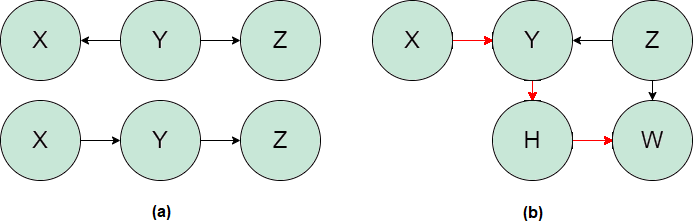
\includegraphics[width=1\linewidth]{chapters/Images/D-SEPARATION.png}
    \caption{Examples of fork and chain structures (a) and of d-separated DAG with a collider between $X$, $Y$ and $Z$ (b)}
    \label{3}
\end{figure}

\begin{definition}[d-separation]\label{d-separation}
    Let $G =(V, E)$ be a DG, $\pi$ be a path on $G$ and $Z$ a subset of $V$. The path $\pi$ is blocked by $Z$ if and only if $\pi$ contains:
    \begin{itemize}
        \item a fork $X \leftarrow Y \rightarrow Z$ or a chain $X \rightarrow Y \rightarrow Z$ such that the middle vertex $Y$ is in $Z$
        \item a collider $X \rightarrow Y \leftarrow Z$ such that middle vertex $Y$, or any descendant of it, is not in $Z$.
    \end{itemize}
\end{definition}

The set $Z$ d-separates $X$ from $Y$ if it blocks every path between $X$ and $Y$ (in \ref{3} (b) example, we have that $X$ and $W$ are d-separated considering the path that includes $Z$, but they become connected if we condition on this latter). When we say that a pair of nodes are d-separated, we mean that the variables they represent are definitely independent; when we say that a pair of nodes are d-connected, we mean that they are possibly, or most likely, dependent.\\

\textbf{\textit{see what to keep here below}}\\
In d-separation, the "d" stands for directional. This criterion offers a set of rules to determine if two variables are independent given a specific set of conditioning variables, which can be either a single variable or a collection of variables. Two variables with a directed edge ($\rightarrow$) between them are dependent. The set of testable implications provided by d-separation can be benchmarked with the available data $D$. If a graph $G$ might have been generated from a dataset $D$, then d-separation tells us which variables in $G$ must be independent conditional on other variables. If every d-separation condition matches a conditional independence in data, then no further test can refuse the model (\cite{pearl1988probabilistic}). If there is at least one path between two variables that is unblocked, then they are d-connected. If two variables are d-connected, then they are most likely dependent (except intransitive cases) (\cite{pearl1988probabilistic}). The d-separation or conditional independence between the variables in the key structures in \ref{fcc} follow some rules which are discussed below:\\
\begin{itemize}
    \item Conditional Independence in Chains: If there is only one unidirectional path between variables $X$ and $Z$, and $Y$ is any variable or set of variables that intercept that path, then $X$ and $Z$ are conditionally independent given $Y$ , i.e. $X \independent Z | Y$ .
    \item Conditional Independence in Forks: If a variable $X$ is a common cause of variables $Y$ and $Z$, and there is only one path between $Y$ and $Z$, then $Y$ and $Z$ are independent conditional on $X$, i.e. $Y \independent Z | X$.
    \item Conditional Independence in Colliders: If a variable $Z$ is the collision node between two variables $X$ and $Y$, and there is only one path between $X$ and $Y$ , then $X$ and $Y$ are unconditionally independent, i.e. $X \independent Y$. But, they become dependent when conditioned on $Z$ or any descendants of $Z$.
\end{itemize}

\begin{definition}[PDAG]
    The graph $G$ is a partially-directed acyclic graph (PDAG) if it can contain both undirected ($-$) and directed ($\rightarrow$) edges.
\end{definition}
\begin{definition}[Skeleton]
    Let $G$ be a PDAG. The skeleton of $G$ is the undirected graph resulting from changing any directed edge of $G$ to undirected.
\end{definition}
\begin{definition}[V-structure]
    Let $G$ be a PDAG. A v-structure in $G$ is a triple $X \rightarrow Y \leftarrow Z$ where $X$ and $Z$ are not adjacent. V-structures are also called unshielded colliders.
\end{definition}
\begin{definition}[Observational equivalence]
    Two DAGs $G$ and $H$ are observationally Markov equivalent if they have the same skeleton and the same V-structures, denoted as $G \equiv H$.
\end{definition}
\begin{definition}[Markov Equivalence Class]
    Two DAGs $G$ and $H$ belong to the same observational Markov equivalence class (MEC) if they are Markov equivalent. As generalization, the MEC of a graph $G$, denoted by $[G]$, represents the set of possible DAGs that are observationally equivalent.
\end{definition}
\begin{definition}[Markov Blanket]
    For any variable X, its Markov blanket (MB) is the set of variables such that X is independent of all other variables given MB. The members in the Markov blanket of any variable will include all of its parents, children, and spouses.
\end{definition}

Other useful definitions.

\begin{definition}[Lagged Causal Effect]
    Lagged Causal Effects refer to causal relationship between variables at the different time points.
\end{definition}
\begin{definition}[Instantaneous Causal Effect]
    Instantaneous Causal Effects refer to causal relationship between variables at the same time point.
\end{definition}
\begin{definition}[Expert knowledge]
    Expert knowledge is a term covering various types of knowledge that can help define or disambiguate causal relations between two or more variables.
\end{definition}
Depending on the context, expert knowledge might refer to knowledge from randomized controlled trials, laws of physics, a broad scope of experiences in a given area, and more.\\

We specify all the assumptions used by the methods in Section \ref{State-of-the-art Methods} to restrict their field of application.\\

\textbf{\textit{Molak e Pearl per approfondimenti e correzioni}}\\

\begin{definition}[Continuous-valued series]
    All series are assumed to have continuous-valued observations.
\end{definition}
However, many interesting data sources - such as social media posts or health states of an individual - are discrete-valued.
\begin{definition}[Causal Markov assumption]
    The causal Markov condition states that the node, V i , is independent of all its non-descendants (excluding its parents) given its parents. Therefore, formally, it can be presented as follows: $$V_i \independent_G \ V_j | PA(V_i) \ \  \forall \ \ j \neq i \in G(V, E) \symbol{92} \{ DE(V_i), PA(V_i) \}, $$ i.e., the node, $V_i$ , is independent of all other nodes in the graph, $G$ , excluding the descendants and parents of this node, given its parents. If this is not entirely clear to you at this stage, that’s perfectly fine.
\end{definition}
\begin{definition}[Linearity]
    The true data generating process, and correspondingly the causal effects of variables on each other, is assumed to be linear.
\end{definition}
 The value assigned to each variable $X_i$ is a linear function of the values already assigned to the earlier variables, plus a ‘disturbance’ (noise) term $e_i$, and plus an optional constant term $c_i$, that is $$X_i = \sum_{k(j)<k(i)} b_{ij}X_j + e_i + c_i$$
In reality, many real-world processes are nonlinear.
\begin{definition}[Discrete time] 
The sampling frequency is assumed to be on a discrete, regular grid matching the true causal time lag.
\end{definition}
If the data acquisition rate is slower or otherwise irregular, causal effects may not be identifiable. Likewise, the analysis of point processes or other continuous-time processes is precluded.
\begin{definition}[Known lag]
    The (linear) dependency on a history of lagged observations is assumed to have a known order. Classically, the order was not estimated and was taken to be uniform across all series.
\end{definition}
\begin{definition}[Stationariety]
    Some statistical properties of the time series do not change over time.
\end{definition}
\begin{definition}[Complete system]
    All relevant variables are assumed to be observed and included in the analysis - i.e., there are no unmeasured confounders.
\end{definition}
\begin{definition}[Absence of selection bias]
    
\end{definition}
\begin{definition}[Absence of feedback configurations]
\end{definition}
\begin{definition}[Sufficiency]
    All relevant variables are measured, and there are no hidden confounders.
\end{definition}
\begin{definition}[Perfectly observed]
     The variables need to be observed without measurement errors.
\end{definition}
\begin{definition}[Faithfulness]
    The observed independencies reflect the true causal structure, we write $$X \independent_P \ Y | Z \rightarrow X \independent_G \ Y | Z, $$ i.e., if $X$ and $Y$ are independent in the distribution given $Z$ , they will also be independent in the graph given $Z$.  
\end{definition}
It’s not very difficult to find situations where the assumption is violated. Intuitively, any situation where one variable influences another through two different paths and these paths cancel each other out completely would lead to the violation of faithfulness.
\begin{definition}[Non-Gaussianity]
    The noise terms are non-Gaussian.
\end{definition}
While the linear-Gaussian approach usually only leads to a set of possible models, equivalent in their conditional correlation structure, a linear-non-Gaussian setting allows the full causal model to be estimated, with no undetermined parameters.
\begin{definition}[No Instantaneous effects]
    Causes do not have immediate effects; there is a time lag between cause and effect.
\end{definition}
\begin{definition}[Time Homogeneity]
    The causal structure does not change over time.
\end{definition}
\begin{definition}[Additivity]
    The effect is a sum of the cause and an independent noise term.
\end{definition}
\begin{definition}[Sparsity]
    The causal graph is sparse, i.e., there are relatively few direct causal connections.
\end{definition}
\begin{definition}[No hidden confounders / Uncorrelated noise variables / Causal sufficience] 
    There are no unobserved variables that affect multiple observed variables; the unobserved noise variables are uncorrelated.
\end{definition}
\begin{definition}[Independence of noise terms]
    The noise terms in different causal mechanisms are independent, $$P(e_1, ..., e_n) = \prod_i P_i(e_i)$$
\end{definition}
\begin{definition}[Temporal order / Causal order]
    The cause precedes the effect in time. No later variable causes any earlier variable.
\end{definition}
\begin{definition}[Acyclicity]
    The causal graph has no cycles (it is a Directed Acyclic Graph, or DAG).
\end{definition}
\begin{definition}[Model Specification]
    The form of the causal relationships (e.g., linear, nonlinear) is correctly specified.
\end{definition}
\begin{definition}[Kernel assumption]
    The relationships can be captured in a high-dimensional feature space using kernel functions.
\end{definition}
\begin{definition}[Consistency]
    The method converges to the correct causal structure as the sample size increases.
\end{definition}
\begin{definition}[Causal minimality]
    The causal minimality assumption states that DAG G is minimal to distribution, P, if and only if G induces P, but no proper sub-graph of G induces P. In other words, if graph G induces P, removing any edge from G should result in a distribution that is different than P.
\end{definition}
Its implications have practical significance for constraint-based causal discovery methods (\ref{Constraint-bsed Methods}) and their ability to recover correct causal structures.
\begin{definition}[Identifiability]
    We say that a causal effect (or any other causal quantity) is identifiable when it can be computed unambiguously from a set of (passive) observations summarized by a distribution $P(V)$ and a causal graph $G$.
\end{definition}
In other words, if we have (1) enough information to control for non-causal information flow in the graph and (2) enough data to estimate the effect of interest, the effect is identifiable.
\begin{definition}[Positivity]
    Positivity assumptions comprehends two conditions: any estimator needs to have a large enough sample size to return meaningful estimates; the probability of every possible value of treatment in our dataset (possibly conditioned on all important covariates) is greater than 0.
\end{definition}
\begin{definition}[Exchangeability / Ignorability]
    The treated subjects, had they been untreated, would have experienced the same average outcome as the untreated did (being actually untreated) and vice versa. Formally: $$\{ Y^0, Y^1 \} \independent \ T|Z.$$ In the preceding formula, $Y^0$ and $Y^1$ are counterfactual outcomes under $T = 0$ and $T = 1$ respectively, and $Z$ is a vector of control variables.
\end{definition}

\textit{Examples from all possible sources}.\\


\section{Causal Inference for Time Series}
Before diving into the state-of-the-art section, it's important to underscore the difference between static and time-varying data (one of the possible cause of distinction in causality framework, as mentioned in \ref{Causality framework exploration}), from which derive two different types of approaches, with their different assumptions.\\

Let's start with the definition of Time Series Data.

\begin{definition}
Time Series data (TS) is a collection of observations measured over consistent
intervals of time. The observation of a Time Series variable $X_{j}$ at time t is denoted by $X^j_{t}$.
\end{definition}\\

Examples of time series data are retail sales, stock prices, climate data, heart rate of patients, brain activity recordings, temperature readings, daily delays of trains for a specific train station, number of ice-cream sold in a month by a supermarket, etc.\\

Discriminating between associative dependencies and effective causal relationships in high-dimensional and temporal settings, like time series data, presents significant challenges in causal inference from observational data. The multivariate interactions in these contexts generate substantial correlations among most variables.(\cite{bontempi2020learning}). 
Considering the potential confounding effects of additional variables is critical to truly discerning the causal relationships within such systems. For example, we can't assess, in a rigorous way, the causal influence of one variable $X_{i}$ on another $X_{j}$ without considering the influence of all other variables in the set $X \symbol{92} {Xi, Xj}$ , where $X$ is the set of all variables considered and the operator $\symbol{92}$ is the subtraction operator. This consideration is crucial because any of these variables, not included in the $(X_i,X_j)$ relationship, could confound it, possibly leading to incorrect conclusions. The unique challenges posed by time series data, due to potential latent confounding factors, are not fully addressed by bivariate models. This has necessitated the development of more sophisticated methods tailored to the complexities of time series analysis. The following section will illustrate some of these methods. (\cite{last paper on TD2C})\\

\textit{\textbf{Add something about it from intros in algos papers}}\\

\begin{figure}[!h]
\centering
\begin{tikzpicture}[
  every node/.style={draw, circle, minimum size=1.5cm, font=\large},
  dashed edge/.style={draw,->,thick, dashed},
  solid edge/.style={draw,->,thick}
]
% Define the nodes
\node (A) at (0,2) {$X^{(t-1)}_i$};
\node (B) at (0,-1) {$X^{(t)}_i$};
\node (C) at (0,-4) {$X^{(t+1)}_i$};
\node (D) at (3,2) {$X^{(t-1)}_j$};
\node (E) at (3,-1) {$X^{(t)}_j$};
\node (F) at (3,-4) {$X^{(t+1)}_j$};
\node (G) at (6,2) {$X^{(t-1)}_z$};
\node (H) at (6,-1) {$X^{(t)}_z$};
\node (I) at (6,-4) {$X^{(t+1)}_z$};
% Define the edges
\path[solid edge, line width=1mm] (A) edge (B);
\path[solid edge, line width=1mm] (B) edge (C);
\path[solid edge, line width=1mm] (D) edge (E);
\path[solid edge, line width=1mm] (E) edge (F);
\path[solid edge, line width=1mm] (G) edge (H);
\path[solid edge, line width=1mm] (H) edge (I);
\path[solid edge] (A) edge (D);
\path[solid edge] (D) edge (G);
\path[solid edge] (B) edge (E);
\path[solid edge] (E) edge (H);
\path[solid edge] (C) edge (F);
\path[solid edge] (F) edge (I);
\path[dashed edge] (B) edge (F);
\path[dashed edge] (A) edge (H);
\path[dashed edge] (A) edge (E);
\path[dashed edge] (E) edge (I);
\path[dashed edge] (D) edge (H);
\path[dashed edge, bend left=30] (A) edge (C);
\path[dashed edge, bend left=30] (D) edge (F);
\path[dashed edge, bend left=30] (G) edge (I);
\end{tikzpicture}
\caption{An example of three time series variables, $X_i$, $X_j$, and $X_z$, connected through a fork structure. The thick solid lines represent the temporal effects of nodes on their immediate subsequent nodes. The thin solid lines represent the contemporaneous effects between nodes of different variables at the same instant. The dashed lines represent the lagged effects between nodes of different variables (or the same variable) at different (or the same) instants.}
\label{TS}
\end{figure}

\chapter{State of the art}\label{State-of-the-art Methods}
In this section we display some of the most valuable strategies for time series causal discovery, their key concepts, their limitations and their applications, in order to create a solid state of the art set of methods we can use to assess the validity of TD2C (\ref{Experiments}).\\

\section{Granger-Based methods}[\textbf{\textit{Maybe to be reduced}}]\\
Let's start our collection of methods with one of the most pivotal concepts in Causal Inference, the Granger Causality.\\

Based on a statistical version of Hume's regularity theory (Hume, 1738), Granger causality is one of the oldest concepts in causal inference. Hume's theory posits that causal relations can be inferred from the consistent conjunction of causes and effects, with causes preceding their effects. Various authors have investigated probabilistic versions of this theory, which rely on the probability-raising principle (conditioning on a cause increases the probability of the effect occurring). The Granger-based family of methods operates on the premise that if past values of one variable help predict the current value of another, they are causally connected. The simplest implementation, the Pairwise Granger causality test, tests the null hypothesis that $X_i$ does not Granger cause $X_j$ (\textbf{cite TD2C paper}). Granger, in 1969, proposed the following definition:

\begin{definition}
    A time series $X^i$ Granger-causes $X^j$ if past values of $X^i$ provide unique, statistically significant information about future values of $X_j$.
\end{definition}

We could also express it in this way:\\
Let $H_{t-1}$ be the history of all relevant information up to time $t-1$ and $P(X_t | H_{t-1})$ be the optimal prediction of $X_t$ given $H_{t-1}$. Granger defined Y to be causal for X if
$$Var(X_t − P(X_t | H_{t-1}) < Var(X_t − P(X_t | H_{t-1}/F^Y_t)$$
where, $H_{t-1}/F^Y_t$ indicates excluding the values of $F^Y_t$ (Filtration of Y, i.e., all Y values up to time t-1) from $H_{t-1}$ . That is, the variance of the optimal prediction error of X is reduced by including the history of Y (informally, Y is causal of X if past values of Y improve the prediction of X). This characterization is clearly based on predictability
and does not (directly) point to a causal effect of Y on X: Y improving the prediction of X does not mean Y causes X. Nonetheless, assuming causal effects are ordered in time (i.e., cause before effect), Granger argued that, under some assumptions, if Y can predict X, then there must be a mechanistic
(i.e., causal) effect; that is, predictability implies causality. \cite{shojaie2022granger}\\

The concept of Granger Causality has been used in the majority of the exciting causal algorithms today (\cite{guo2020survey}). Despite its widespread use, ongoing debate has surrounded the validity of the Granger causality framework for inferring causal relationships among time series. Additionally, while the original definition was broad, the constraints of computational tools have limited the application of Granger causality mainly to simple bivariate vector autoregressive processes (VAR).(\cite{shojaie2022granger}). Let's dig a bit more into this concepts.\\

Granger causality has traditionally relied on assuming a VAR model and considering tests on its coefficients in the bivariate setting.
Denoting the vector of variables at time $t$ by $X_t = (X^1_t , X^2_t , ..., X^p_t)^T$, we consider the linear model $$A^0X_t = \sum_k = 1^d A^kX_{t−k} + e_t$$ where, $A^0, A^1, ..., A^d$ are $p$ × $p$ lag matrices (coefficients) and $d$, the lag, may be finite or infinite. The term $e_t$, $p$-dimensional white noise innovation, or error, can have a diagonal or non-diagonal covariance matrix $\Sigma$. Granger (1969) highlighted that the model generally lacks identifiability because the matrices $A^k$ are not uniquely defined, except when $A^0$ is diagonal. This special case, which aligns with the well-known VAR model, was specifically noted by Granger (\cite{lutkepohl2005new}) — as a “simple causal model,” opposed to models with instantaneous causal effects whose $A^0$ matrix has nonzero off-diagonal values. This latter form is known as a structural vector autoregressive (SVAR) model (\cite{kilian2013structural}) and can be identified under certain parameter restrictions (\cite{kilian2017structural}).\\

As said, in real-world systems involving multiple time series, examining the relationship between only a pair of series can lead to misleading conclusions due to confounding factors. Specific methods, such as like Network Granger causality, are able address this issue by adjusting for potential confounders and considering multiple series simultaneously. Traditional Granger causal analysis, has also several limitations that restrict its broader application. Specifically, the assumptions required for the (S)VAR model to accurately identify Granger causal relationships include continuous-valued series, linearity, discrete time, known lags, stationarity, perfect observation, and a complete system. Since modern time series data often deviate from these assumptions due to nonlinear dynamics and irregular sampling intervals, recent advancements have made it possible to apply Granger causality to a broader range of scenarios by relaxing these assumptions. \cite{shojaie2022granger}\\

Aside from the most popular GC, there are a few other causality concepts in the field such as Sims Causality, and Intervention Causality. The first one is often treated as a compliment of Granger Causality, where Granger Causality implies Sims Causality but the inverse is not true. Sims stated that a pairwise Granger Causality for $X_t$ and $Y_t$ can be treated as moving average along several lag terms of the two variables, expressed as
$$Y_t = \alpha_1 Y_{t-1} + \beta_1 X_{t-2} + ... + \alpha_k Y_{t-k} + \beta_k+1 X_{t-2} + C + \epsilon$$
where, $k$ represents the combined noise term from both variables. $\alpha$ and $\beta$ terms represent the parameter values at each time lag while $C$ is the combined constant term. Sims Causality stated that variable $X$ does not Granger Cause $Y$ if and only if $\beta_1, \beta_2, ..., \beta_k$ is being chosen identically to zero.

Sims' characterizations, which can be shown to be equivalent to Granger's one, can be tested using an F-test comparing two models: the full model, including past values of both x and y, and the reduced model, including only past values of x. We have $$F = \frac{(RSS_{red} - RSS_{full})/(r-s)}{RSS_{full}/(T-r)}$$
where, $RSS_{full}$ and $RSS_{red}$ are the residual sum of squares for the full and reduced models with $r$ and $s$ parameters, respectively. Using this test, Y is declared Granger causal for X if the observed test statistic $F$ exceeds the (1 − $\alpha$)\% quantile of an $F$-distribution with $r - s$ and $T - r$ degrees of freedom. (\cite{shojaie2022granger})\\

Another causality interpretation, that we call Intervention Causality was proposed by Judea Pearl in 1993 and has been applied to TS data recently. This conception focuses on the idea of counterfactual and calculates the Average Causal Effect (ACE) $$ACE_S = E(Y_{t^*}) - E(Y_t)$$
where, $E(Y_{t^*})$ represents the resulting outcome for variable $Y$ at time $t$ given the occurrence of intervention $S$ and $E(Y_t)$ represents the expected outcome for variable $Y_t$ without the intervention. While concepts such as Granger Causality and Sims Causality assume an observational framework, Intervention Causality requires counterfactual experiments which are not applicable in many real world applications. Our TD2C algorithm falls into the first group. \cite{chang2021multivariate}\\

\section{The 4, 5, 6, ... Families}
In the current literature, there are numerous Causal Discovery methods for both static and time series data. Each method offers unique benefits and faces specific challenges, but the boundaries between them can often be not evident (\cite{hasan2023survey}). Some of these families find application for both types of data, with an obvious more large difficulty for the time-depending ones. In this section we limit our interest in the families whose methods are able to handle successfully this time dependency, and whose application has so far brought at significant results. These methods, as we will see, need to fit in the assumption-wise restricted frame of TD2C method, in order to have a fair and relevant evaluation of this latter.\\
The families we are going to define are the Constraint-based, the Noise-based, the Gradient-based and the Tidybench Methods. The remaining families include all the hybrid methods and other methods that do not fit our main four categories: Score-based (only valid for IID data, i.e., static data), Kernel-based (from which D2C's logic derives it inspiration), Logic-based, Topology-based, Difference-based, ecc. In Figure \ref{fig:2} we summarize schematically what just said.\\

\begin{figure}
    \centering
    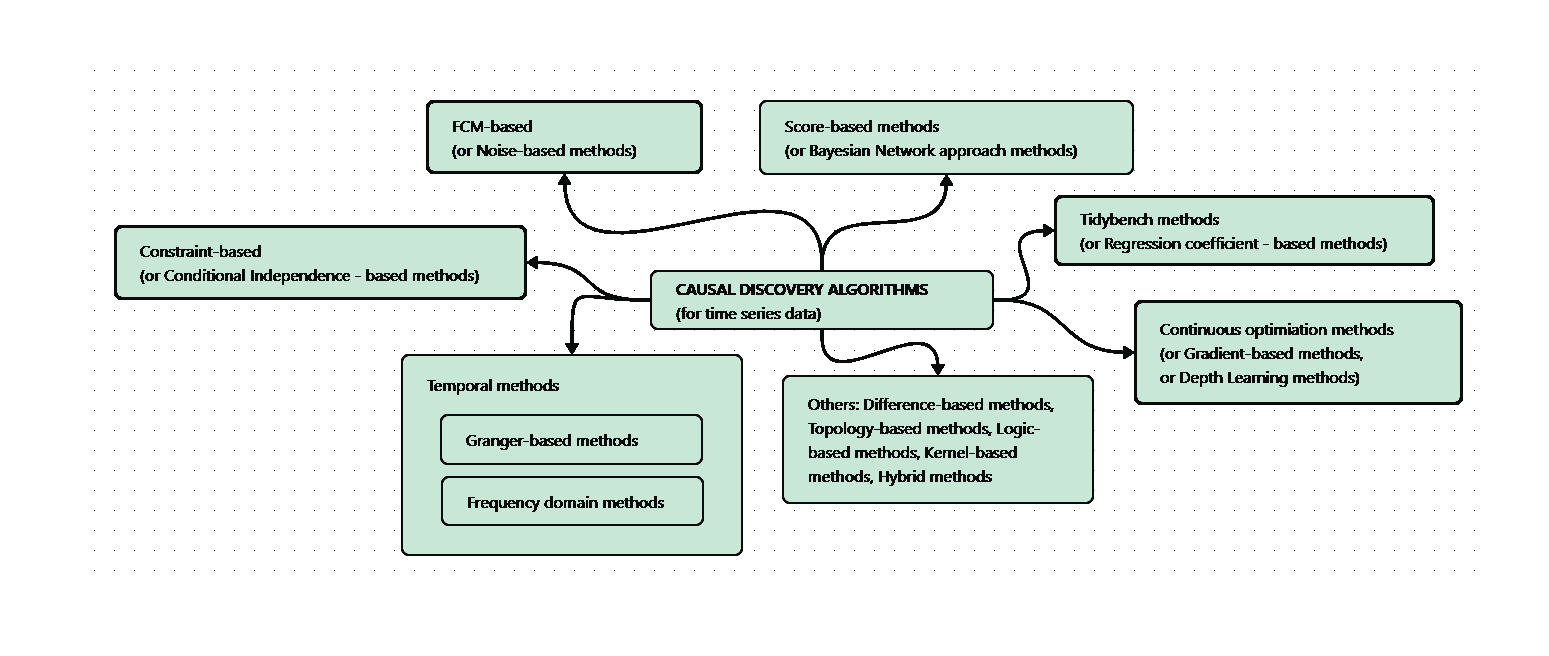
\includegraphics[width=1\linewidth]{chapters/Images/Causal Discovery methods.png}
    \caption{Scheme of the most known Causal Discovery methods (in blue, the families we are going to use as benchmarks in the experiments)}
    \label{fig:2}
\end{figure}

\subsection{Contraint-based Methods}\label{Constraint-bsed Methods}
Constraint-based methods in causal discovery rely on graph independencies (\cite{molak2023causal}). A key goal of these methods is testing for conditional independence (CI), which helps recover the causal skeleton when the observed data’s probability distribution is faithful to the underlying causal graph.\cite{runge2020discovering} These approaches aim to determine the presence or absence of edges in the data through the d-separation criterion, i.e. by identifying variables that are d-separated or d-connected. By employing CI tests, constraint-based methods recover the Markov equivalence class of DAGs, assuming faithfulness. Despite their speed, these methods are sensitive to the graph structure and prone to error propagation (\cite{hasan2023survey}).
Some of the most used CB methods are in table \ref{CBm}.

\begin{table}[!ht]
    \centering
    \caption{Table of the most known Constraint-based methods in the literature}
    \begin{tabular}{|l|l|}
    \hline
        \textbf{IID Data} & \textbf{TS Data} \\ \hline
        PC & tsFCI \\ \hline
        FCI & \textcolor{RoyalBlue}{PCMCI} \\ \hline
        ANYTIME FCI & PCMCI+ \\ \hline
        RFCI & LPCMCI \\ \hline
        PC-STABLE & CD-NOD \\ \hline
        PKCL & CDANs \\ \hline
    \end{tabular}
    \label{CBm}
\end{table}

%A problem with large-scale time series data is that although adding more variables makes causal analysis more interpretable, if the additional variables don’t have a significant effect on the causal model, this, in turn, makes the analysis less powerful, and original causal relations may also be overlooked. Moreover, at large dimensions, certain nonlinear tests even lose their ability to limit false positive rates (FPRs). \\

PCMCI is building upon the foundational principles of the PC algorithm. This latter operates operates in three steps: first, identifying the skeleton of the graph by starting with a fully connected undirected graph and then eliminating unconditionally and conditionally independent edges; second, determining V-structures or colliders (e.g., $X \rightarrow Y \leftarrow Z$) using the d-separation set of node pairs; and third, orienting the remaining edges to avoid new V-structures and cycle formation. This process results in a CPDAG, which represents the underlying causal DAG.\\

PCMCI, proposed by Runge et al. (2019), adapts the PC algorithm for time series data, addressing its limitations. It assumes stationarity, causal sufficiency, and the presence of time-lagged dependencies. The algorithm operates in two main stages. In the first stage, it employs PC1, a variant of the skeleton discovery phase of the PC algorithm, to remove irrelevant variables. In the second stage, the algorithm uses the Momentary Conditional Independence (MCI) test to assess whether two variables are independent given their parent sets: $$X^i_{t - \tau} \independent X^j_t | P_A(X^j_t), P_A(X^i_{t - \tau})$$  \cite{hasan2023survey}.

Even when the assumption of stationarity is violated, typically due to obvious confounders, PCMCI still performs more robustly compared to Lasso regression or the PC algorithm. However, PCMCI is less effective for highly predictable systems where little new information is produced at each time step. One significant issue with PCMCI is autocorrelation, which PCMCI+, a more recent version attempts to address. (\cite{runge2020discovering})

\subsection{Gradient-based Methods}
Gradient-based methods stem from research that treats the graph space search as a continuous optimization problem \cite{molak2023causal}. Recent advancements in causal discovery have redefined the structure learning problem as a continuous optimization task, employing a least squares objective alongside an algebraic characterization of Directed Acyclic Graphs (DAGs). This approach transforms the combinatorial structure learning problem into a continuous one, solvable through gradient-based optimization techniques. To further expedite the process, deep learning models capable of capturing intricate nonlinear mappings are often employed. Consequently, these models generally exhibit faster training times, as deep learning is known for its high degree of parallelism on GPUs. They update all edges at each step, considering both the gradient of the score and the acyclicity constraint. \cite{hasan2023survey}\\

\begin{table}[!ht]
    \centering
    \caption{Table of the most known Gradient-based methods in the literature}
    \begin{tabular}{|c|c|c|c|c|}
    \hline
        \textbf{IID Data} & NOTEARS & DAE & GOLEM & MCSL \\ \hline
        \multicolumn{1}{c|}{} & GraN-DAG & DAG-GNN & DAG-NoCurl & ENCO \\ \hline
        \textbf{TS Data} & \textcolor{RoyalBlue}{DYNOTEARS} & NTS-NOTEARS & ~ & ~ \\ \hline
    \end{tabular}
    \label{gbM}
\end{table}

Pamfil et al. (\cite{pamfil2020dynotears}), in 2020, introduced the Dynamic NOTEARS (DYNOTEARS) approach, which is designed for structure learning in dynamic data. DYNOTEARS extends the static NOTEARS method to handle both contemporaneous (intra-slice) and time-lagged (inter-slice) dependencies in dynamic Bayesian networks (DBNs). This methodology involves minimizing a penalized loss function while ensuring that the resulting graph structure is acyclic. The acyclicity constraint is enforced using an algebraic condition that characterizes acyclicity in directed graphs. The method assumes that the structure of the network remains constant over time and is the same across all time series. This fixed-structure assumption simplifies the problem and allows DYNOTEARS to scale effectively to high-dimensional datasets. The approach does not impose implicit constraints on the underlying graph. \cite{hasan2023survey}\\

The model used in DYNOTEARS is a Structural Vector Autoregressive (SVAR) model, where each time series is represented as $X^T_{m,t} = X^T_{m,t}W + X^T_{m,t-1}A_1 + ... + X^T_{m,t-p}A_p + Z^T_{m,t}$ for $t \in {p, ..., T}$ and for all $m \in {1, ..., M}$.. Here, $W$ captures contemporaneous relationships, while $A_1, ..., A_p$ represent time-lagged dependencies. This can be expressed in matrix form as $X = XW + Y_1A_1 + ... + Y_pA_p + Z$, where $X$ is the matrix of observations, $Y$ represents time-lagged versions of $X$, and $Z$ denotes the error terms. The optimization problem tackled by DYNOTEARS involves minimizing the penalized loss function $f(W,A) = \frac{1}{2n}||X - XW - YA||^2_F + \lambda_A||A||_1$ subject to the constraint that $W$ is acyclic. The acyclicity constraint is given by $h(W) = tr(e^{WoW}) - d = 0$, where $o$ denotes the Hadamard product. To solve this optimization problem, DYNOTEARS employs the augmented Lagrangian method, transforming the constrained problem into a series of unconstrained subproblems that can be addressed with standard solvers.\\


\subsection{Noise-based Methods (Functional Methods)}
Drawing inspiration from Independent Component Analysis (ICA), a range of algorithms focuses on unraveling the causal relationships among variables by examining their functional dependencies \cite{molak2023causal}. These algorithms often operate within the framework of Functional Causal Models (FCMs), which articulate the causal connections between variables through specific functional forms. In FCMs, each variable is modeled as a function of its direct causes, accompanied by an independent noise term. This is captured by the equation $$X = f(PA_X) + E$$, where $f$ represents the functional dependency on the parent variables $PA_{X}$, and $E$ denotes the stochastic noise component. By incorporating additional constraints on data distributions or function classes, FCM-based approaches can differentiate between various Directed Acyclic Graphs (DAGs) that belong to the same equivalence class. This capacity to distinguish among DAGs is essential for refining causal inferences and understanding the underlying mechanisms driving the observed data. \cite{hasan2023survey}\\

\begin{table}[!ht]
    \centering
    \caption{Table of the most known Noise-based methods in the literature}
    \begin{tabular}{|c|c|c|c|c|}
    \hline
        \textbf{IID Data} & LiNGAM & ANM & PNL & Direct-LiNGAM \\ \hline
        \multicolumn{1}{c|}{}  & SAM & CGNN & CAM & CAREFL \\ \hline
        \textbf{TS Data} & \textcolor{RoyalBlue}{VarLiNGAM} & TiMINo & ~ & ~ \\ \hline
    \end{tabular}
    \label{nbM}
\end{table}

To uncover the complete causal structure from continuous-valued data, the Linear Non-Gaussian Acyclic Model (LiNGAM) framework is utilized, capitalizing on the independence of non-Gaussian disturbance terms and the linearity of the data-generating process. This approach assumes a recursive causal model, where observed variables are influenced linearly by earlier variables plus non-Gaussian disturbances, without any unobserved confounders (VarLiNGAM also asssumes acyclicity of contemporaneous causal relations). \cite{shimizu2006linear}\\

The core methodology involves Independent Component Analysis (ICA) to identify the underlying causal structure. In a LiNGAM framework, observed data $X$ can be expressed as $X = BX + E$, where $B$ represents the matrix of connection strengths among variables, and $E$ contains the independent, non-Gaussian disturbances. By applying ICA, the model transforms $X = AE$, where $A$ is derived from $(I-B)^{-1}$. ICA's capability to exploit non-Gaussianity allows for a precise estimation of $A$, overcoming the limitations inherent in Gaussian settings where different mixing matrices can yield identical covariance structures. The ICA-based approach does face challenges like the indeterminacies of component order and scaling, but these can be managed by normalizing components and adjusting the matrix $W = A^{-1}$, involved in the 5-steps algorithm. \cite{shimizu2006linear}\\

Building on these principles, the VarLiNGAM algorithm extends the LiNGAM approach by incorporating autoregressive components. This method integrates non-Gaussian instantaneous models with vector autoregressive (VAR) models to estimate both immediate and lagged causal effects. The VarLiNGAM algorithm highlights the importance of accounting for instantaneous influences, as neglecting them can significantly skew the interpretation of time-lagged causal relationships. It demonstrates that, even without prior knowledge of network structure, a non-Gaussian model can be effectively identified, enhancing the accuracy and reliability of causal inference in complex temporal systems. \cite{hasan2023survey}


\subsection{Tidybench Methods (Regression Coefficient-based Methods)}
\textit{\textbf{Evalueate if considering these methods}}\\
- SLARAC, QRBS, LASAR, SELVAR\\

\textit{\textbf{Other eventual Methods relevant for the analysis...}}

\section{D2C \& caD2C}
Finally, we reached the section dedicated to the protagonist of this study, the D2C method. Here we explain its logic and its evolution in the last ten years.\\

\subsection{Introduction to D2C}\label{introd2c}
D2C's main idea has been introduced in 2015 (Bontempi \& Flausder, \cite{bontempi2015dependency}): it's a data driven approach that apply supervised machine learning to infer the causality connections within a multivariate ($n>2$) set of variables. Its main idea relies on the asymmetry generated by two causally related variables that can be noticed in the distribution of their their Markov Blankets' connected variables. It uses some descriptors able to capture this asymmetry and a classifier which learns from artificial data how to discriminate between causal and non causal relations using such descriptors. From its first version (2015), some modifications of the method have been proposed (\cite{bontempi2020learning}, \textbf{\textit{TD2C paper}}) to overcome certain limitations that we will mention later. Anyway, the logic behind the algorithm has remained the same. It is part of the probabilistic methods, (i.e. which infer the probability of existence of a causal link between two variables and then its directionality) relying on observational data, which uses a supervised machine learning approach whose inputs are features able to describe variables' dependency. This ability to reduce uncertainity about the causal relationships using statistical features is common to methods such as ANM (Additive Noise Models), IGCI (Information Geometry Causality Inference), LiNGAM and others. These are able to bypass indistinguishability, which limits the functioning of methods relying on conditional independence (CI) tests, such as Constraint-based approaches. D2C has the merit to expand the field of application of these approaches to multivariate data, a much more complicated operation due to growing parameters and causal interactions.\\
This method is able to derive the relationships between the $n$ variate distribution $X =$ $(X_1,$ $X_2,$ $...,$ $X_n)$ and the existence of a directed causal link between two variables $X_i$ and $X_j$, for $1 \leq i \neq j \leq n$, assuming no confounding, no selection bias and no feedback configurations. 
For the features, it uses structural quantitative characteristics of the data, with the same asymmetry properties, based on information theory concepts (used to quantify the notion of conditional independence), able to derive causality from dependency. Let's see more in detail how the process works in the next section.\\

\subsection{Causality as an asymmetric distribution}
Here we report the mathematical tools that allow us to recognise that asymmetry we mentioned above and to create features able to describe it.\\

First, we need to define dependency
\begin{definition}[Dependency]
    A variable $X_i$ is dependent on a variable $X_j$ if $$p(X_i|X_j = x_j) \neq p(X_i)$$ and we write $X_i \dep X_j$.
\end{definition}
Dependency is symmetric, so, if $X_i \dep X_j \Rightarrow X_j \dep X_i$.\\

Then, we need to define mutual information, and we do it in form of probabilistic density functions:
\begin{equation} \label{eq1}
    I(X_1; X_2) = \int \int log\frac{p(X_1, X_2)}{p(X_1)p)(X_2)}p(X_1, X_2)dX_1dX_2 = H(X_1) - H(X_1|X_2)
\end{equation}
where $H$ is the entropy and we use the convention $0 \ log \ \frac{0}{0}$. This formula measures the amount of stochastic dependence between $X_1$ and $X_2$.\\ 

Dependency becomes, in information terms: $I(X_i; X_j) = I(X_j; X_i) > 0$. It follows that, speaking of conditional mutual information, $I(X_i;X_j|X_z) = 0 \ $ if $ \ p(X_i,X_j|X_z) = p(X_i|X_z)p(X_j|X_z)$, i.e. \textbf{Conditional mutual information between two variables $\bm{X_i}$ and $\bm{X_j}$, given another variable $\bm X_z$, is null if $\bm{X_i}$ and $\bm{X_j}$ are conditionally independent given $\bm{X_z}$, i.e. $\bm X_i \bm\dep \bm X_j \bm| \bm X_z$} (as well as ${I(X_1; X_2) = 0}$ if ${p(X_1, X_2) = p(X_1)p(X_2)}$). The link between this notion and our causality problem is the definition of Markov Blanket:$$I(X_i;(X \symbol{92} (M_i \cup X_i))|M_i) = C_i \cup E_i \cup S_i = 0,$$ where $C_i = {X_c|X_c \rightarrow X_i}$ is the set of variables that have direct arrows pointing to $X_i$ (causes), $E_i = {X_e|X_i \rightarrow X_e}$, are the set of variables to which $X_i$ has a direct causal influence, i.e., where $X_i$ is the parent (effects) and $Si = \{X_s| \ \exists \ X_j : Xs \rightarrow Xj \leftarrow Xi$ and $Xs \neq Xi\}$, are the variables that are not direct causes or effects of $X_i$ but are connected to $X_i$ through a common effect (spouses).\\

Finally, thanks to the \textit{do-operator}, we can define causality, which, instead, is not symmetric in a probabilistic way: We consider, for example, the causal link $X_i \rightarrow X_j$ and we have that $$p(X_j|do(X_i = x_i)) \neq p(X_j), \ but, \ convercely, \ $$  $$p(X_i|do(X_j = x_j)) = p(X_i).$$ Here stands the asymmetry in distribution (Figure \ref{do-}).\\

\

Another way to define causality is graphically, by using a faithful DAG and the rules of d-separation (Figure \ref{fig1}).\\

\begin{figure}[!h]
\centering
\begin{tikzpicture}[
  every node/.style={draw, circle, minimum size=1.5cm, font=\large},
  dashed node/.style={draw, circle, minimum size=1.5cm, dashed, font=\large},
  dashed edge/.style={draw,->,thick, dashed},
  solid edge/.style={draw,->,thick}
]
% Define the nodes
\node[fill=Emerald, text=white] (A) at (2,2) {$X_i$};
\node[fill=Emerald, text=white] (B) at (6,-3) {$X_j$};
\node (C) at (1,4) {$C^{(1)}_i$};
\node (D) at (2,-1) {$E_i$};
\node (E) at (0,1) {$S_i$};
\node (F) at (5.5,0) {$C^{(1)}_j$};
\node (G) at (6,-6) {$E_j$};
\node (H) at (4,-4) {$S_j$};
\node[dashed node] (I) at (-1.5,4.5) {$A_i$};
\node[dashed node] (J) at (-1.5,-3) {$D_i$};
\node (K) at (3,4.5) {$C^{(2)}_i$};
\node (L) at (7.5,0.5) {$C^{(2)}_j$};
% Define the edges
\path[solid edge, line width=1mm] (A) edge (B);
\path[solid edge] (C) edge (A);
\path[solid edge] (A) edge (D);
\path[solid edge] (E) edge (D);
\path[solid edge] (F) edge (B);
\path[solid edge] (B) edge (G);
\path[solid edge] (H) edge (G);
\path[dashed edge] (I) edge (C);
\path[dashed edge] (D) edge (J);
\path[dashed edge] (I) edge (J);
\path[solid edge] (K) edge (A);
\path[solid edge] (L) edge (B);
\end{tikzpicture}
\caption{ Two causally connected variables ($X_i$ and $X_j$) and their Markov Blankets}
\label{fig1}
\end{figure}

As last, we need to define the descriptors that will be used to train the classifier. We surely need asymmetric measures (not as correlation or mutual information, which are dependency measures, i.e., symmetric: $\rho(i,j) = \rho(j,i)$, $I(i,j) = I(j,i)$). To find such descriptors we rely on the elements in the MBs of the two variables ($M_i, M_j$): $S, C$ and $E$. Thanks to two assumptions: 
\begin{enumerate}
    \item The only path between the sets $X_i \cup M_i$ and $X_j \cup M_j$ is the edge $X_i \rightarrow X_j$.
    \item There are no common ancestors betwween $X_i(X_j)$ and its spouses $S_i(S_j),$
\end{enumerate}
\textbf{\textit{(DOUBT: how to verify these conditions in real-world data)}}

we are able to recognise asymmetric conditional independence relationships between $M_i$ and $M_j$ (Table \ref{table1}(a)), which bring to asymmetric mutual information measures (Table \ref{table2}(a)).\\  

\begin{table}[!ht]
    \centering
    \caption{($\forall k$) All symmetric (b) and asymmetric (a) (un)conditional (in)dependence relationship between $M_i$ and $M_j$ members from \ref{fig1}. Relations $S - C$ and $S - S$ are not considered because they include particular relations, not essential for our goal.}
    \label{table1}
    \begin{tabular}{cc}
        \begin{subtable}[t]{0.45\textwidth}
            \centering
            \caption{ }
            \begin{tabular}{l|l}
            \hline
                \textbf{i - j relations} & \textbf{j - i relations} \\ \hline 
                $X_i \dep C^{k}_j|X_j$ & $X_j \independent C^{k}_i|X_i$ \\ 
                $E_i \dep C^{k}_j|X_j$ & $E_j \independent C^{k}_i|X_i$ \\ 
                $C_i \dep C^{k}_j|X_j$ & $C_j \independent C^{k}_i|X_i$ \\
                $X_i \independent C^{k}_j$ & $X_j \dep C^{k}_i$ \\
                $E_i \independent C^{k}_j$ & $E_j \dep C^{k}_i$ \\ \hline
            \end{tabular}
        \end{subtable} & 
        \begin{subtable}[t]{0.45\textwidth}
            \centering
            \caption{ }
            \begin{tabular}{l|l}
            \hline
                \textbf{i - j relations} & \textbf{j - i relations} \\ \hline
                $X_i \independent E^{k}_j|X_j$ & $X_j \independent E^{k}_i|X_i$ \\ 
                $X_i \independent S^{k}_j|X_j$ & $X_j \independent S^{k}_i|X_i$ \\ 
                $E_i \independent E^{k}_j|X_j$ & $E_j \independent E^{k}_i|X_i$ \\
                $E_i \independent S^{k}_j|X_j$ & $E_j \independent S^{k}_i|X_i$ \\
                $X_i \dep E^{k}_j$ & $X_j \dep E^{k}_i$ \\
                $X_i \independent S^{k}_j$ & $X_j \independent S^{k}_i$ \\
                $E_i \dep E^{k}_j$ & $E_j \dep E^{k}_i$ \\
                $E_i \independent S^{k}_j$ & $E_j \independent S^{k}_i$ \\
                $C_i \independent C^{k}_j$ & $C_j \independent C^{k}_i$ \\ \hline
            \end{tabular}
        \end{subtable} \\
    \end{tabular}
\end{table}

\begin{table}[!ht]
    \centering
    \caption{($\forall k$) All symmetric (b) and asymmetric (a) (un)conditional mutual information between $M_i$ and $M_j$ members from \ref{fig1}. Relations $S - C$ and $S - S$ are not considered because they include particular relations, not essential for our goal.}
    \label{table2}
    \begin{tabular}{cc}
        \begin{subtable}[t]{0.45\textwidth}
            \centering
            \caption{ }
            \begin{tabular}{l|l}
                \hline
                \textbf{i - j relation} & \textbf{j - i relation} \\ \hline
                $I(X_i;C^{k}_j|X_j) > 0$ & $I(X_j; C^{k}_i|X_i) = 0$ \\ 
                $I(E_i;C^{k}_j|X_j) > 0$ & $I(E_j; C^{k}_i|X_i) = 0$ \\ 
                $I(X_i;C^{k}_j|X_j) > 0$ & $I(C_j; C^{k}_i|X_i) = 0$ \\
                $I(C_i; C^{k}_j) = 0$ & $I(X_j \dep C^{k}_i) > 0$ \\
                $I(E_i; C^{k}_j) = 0$ & $I(E_j \dep C^{k}_i) > 0$ \\ \hline
            \end{tabular}
        \end{subtable} & 
        \begin{subtable}[t]{0.45\textwidth}
            \centering
            \caption{ }
            \begin{tabular}{l|l}
                \hline
                \textbf{i - j relation} & \textbf{j - i relation} \\ \hline
                $I(X_i;E^{k}_j|X_j) = 0$ & $I(X_j; E^{k}_i|X_i) = 0$ \\ 
                $I(X_i;S^{k}_j|X_j) = 0$ & $I(Z_j; S^{k}_i|X_i) = 0$ \\ 
                $I(E_i;E^{k}_j|X_j) = 0$ & $I(E_j; E^{k}_i|X_i) = 0$ \\
                $I(E_i;S^{k}_j|X_j) = 0$ & $I(E_j; S^{k}_i|X_i) = 0$ \\
                $I(X_i; S^{k}_j) = 0$ & $I(X_j \dep S^{k}_i) = 0$ \\
                $I(E_i; S^{k}_j) = 0$ & $I(E_j \dep S^{k}_i) = 0$ \\
                $I(C_i; C^{k}_j) = 0$ & $I(C_j \dep C^{k}_i) = 0$ \\
                $I(E_i; E^{k}_j) > 0$ & $I(E_j \dep E^{k}_i) > 0$\\
                $I(X_i; E^{k}_j) > 0$ & $I(X_j \dep E^{k}_i) > 0$ \\
                 \hline
            \end{tabular}
        \end{subtable} \\
    \end{tabular}
\end{table}


The problem is that to know this relationships we need to already know which are the causes, the effects and the spouses in $M_i$ and $M_j$, which is the same information we are trying to derive.\\

To solve this problem, we rely on the following: considering the two MB as mixtures of three distributions (for E, S and C) and knowing that there is an asymmetry within there three described by elements in \ref{table1}(a), even without knowing exactly which role each element assumes (E, S or C), we know the two mixtures are different.\\
Observing the elements in \ref{table2} we notice that, for example, $$
\begin{cases}
    I(X_i;m^{kj}_j|X_j) > I(X_j;m^{ki}_i|X_i) = 0  \ \ \ \ \ \ \ \ if \ \ m^{kj} = C^{kj}_j \ \wedge \  m^{ki} = C^{ki}_i \\
    I(X_i;m^{kj}_j|X_j) = I(X_j;m^{ki}_i|X_i) = 0 \ \ \ \ \ \ \ \ else
\end{cases}
$$
where $m^{ki}$ ($m^{kj}$) is a member of $M_i$ ($M_j$) and we are taking the mixtures of the kind $D_1(i,j) = \{I(X_i; m^{(kj)}_j|X_j)$, $k_j = 1, ..., K_j$\} and $D_1(j,i) = \{I(X_j; m^{(ki)}_i|X_i$), $k_i = 1, ..., K_i$\}. So, as said, the populations $D_1(i,j)$ and $D_1(j,i)$ are different, and we can use them (or some of their moments) as our descriptors of causal dependency. In Table \ref{table3} we put all the asymmetric mixtures D.

\begin{table}[!ht]
    \centering
    \begin{tabular}{l}
    \hline
        \textbf{Asymmetric mixtures} \\ \hline
         (a) $D_1(i,j) = \{I(X_i; m^{(kj)}_j|X_j)$, $k_j = 1, ..., K_j$\}\\
         (b) $D_1(j,i) = \{I(X_j; m^{(ki)}_i|X_i)$, $k_i = 1, ..., K_i$\}\\
         (c) $D_2(i,j) = \{I(m^{(ki)}_i; m^{(kj)_j}|X_j)$, $k_i = 1, ..., K_i$, $k_j = 1, ..., K_j$\}\\
         (d) $D_2(j,i) = \{I(m^{(kj)}_j; m^{(ki)_i}|X_i)$, $k_i = 1, ..., K_i$, $k_j = 1, ..., K_j$\}\\
         (e) $D_3(i,j) = \{I(X_i;m^{(kj)}_j)$, $k_j = 1, ..., K_j$\}\\ (f) $D_3(j,i) = \{I(X_j;m^{(ki)}_i)$, $k_i = 1, ..., K_i$\}
         \\ \hline
    \end{tabular}
    \caption{Asymmetric mixtures from which all the causal descriptors will be generated}
    \label{table3}
\end{table}


\subsection{The algorithm}\label{d2c}
The algorithm starts from two sets of features: one is used to infer the MBs of the two considered variables ($X_i, X_j$) through a filter algorithm (could be mIMR), which also creates a previous relevance ranking within $M_i$ and $M_j$'s elements (we saw that $C$ (causes) elements are much more informative on the direction or causal effects with respect to E (effects) and S (spouses) ones); the other is made by a set of quantiles that summarise the asymmetric mixtures distributions found in the previous section (\ref{table3}). The combined dataset, intended for the classifier, is made of vectors ($d = (d_1, ..., d_i, ..., d_p)$) composed by: a set of mutual information terms between $X_i$ and $X_j$ (estimated as difference of entropy terms, as in \ref{eq1}, through a Lazy Learning algorithm under Gaussian noises assumption), the positions (in the ranking created previously) $P^{ki}_i$ ($P^{kj}_j$) of members $m^{ki}_i$ ($m^{ki}_i$) of $M_i \symbol{92} X_j$ ($M_j \symbol{92} X_i$), the quantiles describing populations in Table \ref{table3} and a binary response variable, \textit{Class}, that indicates the presence (1) or the absence (0) of the causal link. Synthetic dataset of this kind, with complexity $O(Cn + Cn^{'2} + K_iK_jN)$ (\textbf{\textit{specify meanings}}) for each test between two variables, are generated and then used by a Random Forest classifier which, as last step, produces a classification on a testset for validation. In Figure \ref{proc} you can find a graphical representation of the whole process.\\

\textbf{\textit{Insert the formalized algorithm}}.
    % Definizioni formali del problema 
    % Metodi che affrontano il problema 
    % D2C

\chapter{Methods}
\section{Latest updates - TD2C}
As said in \ref{introd2c}, D2C was introduced in \cite{bontempi2015dependency}. Later on, with \cite{bontempi2020learning} and \textbf{\cite{TD2C paper}}, certain aspects of the original procedure have been changed to solve some of the problematics (e.g. computational cost). \\

At firs, the authors introduced a new descriptor, aiming to featurize the context, based on the notion of interaction information: $$I(m^{(1)}_i;m^{(2)}_i;X_i) = I(m^{(1)};m^{(2)}_i;X_i) - I(m^{(1)}_i;m^{(2)}_i|X_i),$$ which gives insights on the causal links characterizing the considered data (in particular, positive interactions derive from common effect configurations, while negative ones form common cause configurations), in order to derive an appropriate DAG structure. The underlying context is maybe more clear in Figure \textbf{\textit{inserire figura}}, where given the latent nature of the nodes F and G, no d-separation (i.e. no independence) occurs between the nodes B,C,D,E and the node A. This means that the features associated to the nodes B,C,D,E are informative about the state of the node A. In other words, by measuring the quantities represented by nodes B,C,D,E we may reduce the uncertainty about the binary state of the node A. \textbf{\textit{figure3}}. As a result, the ranking procedure described in \ref{d2c} is simplified (no more bootstrapping is needed, instead, a correlation to the target measure is used), and complexity for each pair $X_i$ - $X_j$ becomes $O(Cn + K^2N)$.\\
This addition wanted to show that context aware learning approaches, as the ones based on Granger causality (methods based on the precedence concept, which is an associative measure not a causal one and so usually utilized to infer strong relevance and not causality), are adequate to infer causal relationships in large variate contexts, as for multivariate TS. This first modification is in \cite{bontempi2020learning} and is called caD2C ("context aware").\\

The last update (\textbf{\cite{TD2C paper}}) of the method proposes some variations to better leverage the temporal dependencies of time series data and reduce the dimensionality of the problem.
Starting from the same set of assumptions as before: absence of confounding, selection bias, and feedback configurations, faithfulness, stationarity and lagged effects ($X^{(t-1)}_i \rightarrow X^{(t)}_i \ \forall \ (i, t)$), it proposes the followings:
\begin{itemize}
    \item Thanks to the lagged effects assumption, it is able to reduce the relevant members of a considered MB, i.e. to reduce dimensionality, and so to skip the MB estimation phase of \cite{bontempi2015dependency}.
    Looking at the simplified example in Figure \ref{TS}, we see that, studying the causal link $X^{(t)}_i \rightarrow X^{(t+1)}_j$ and only considering effects and causes for them, we can reduce the asymmetric mixtures seen in Table \ref{table1} to the ones in Table \ref{table4} 
    \item Adopts the knnCMI method to estimate conditional mutual information using a nearest neighbors approach, differently from \cite{bontempi2020learning}, where a prediction error from a regression model was informing the entropy estimation under the Gaussian assumption.
    \item precise which descriptors are used
    \item precise all the data generating process and so how complexity changes
\end{itemize}

\begin{table}[!ht]
    \centering
    \caption{Shrinked set of descriptors used by TD2C}
    \begin{tabular}{c|c}
    \hline
        \textbf{CMI terms \ \ $\forall \ \ (m^{(k_i)}_i, m^{(k_j)}_j)$} & \textbf{Families of asymmetric mixtures} \\ \hline
        ~$I(X_i; m^{(k_j)}_j|X_j)$ & $D_{xmx}(i,j) = I(X^{(t)}_i; m^{(k_j)}_j|X^{(t+1)}_j)$, $m^{(k_j)}_j \in \{X^{(t+2/t)}\}$~ \\
        ~$I(X_j; m^{(k_i)}_i|X_i)$ & $D_{xmx}(j,i) = I(X^{(t+1)}_j; m^{(k_i)}_i|X^{(t)}_i)$, $m^{(k_i)}_i \in \{X^{(t-1/t+1)}\}$~ \\
        ~$I(m^{(k_i)}_i; m^{(k_j)}_j|X_i)$ & $D_{mmx}(i,j) = I(X^{(t-1/t+1)}_i; m^{(k_j)}_j|X^{(t)}_i)$, $m^{(k_j)}_j \in \{X^{(t/t+2)}\}$~ \\
        ~$I(m^{(k_j)}_j; m^{(k_i)}_i|X_j)$& $D_{mmx}(j,i) = I(X^{(t/t+2)}_j; m^{(k_i)}_i|X^{(t+1)}_j)$, $m^{(k_i)}_i \in \{X^{(t-1/t+1)}\}$~ \\ \hline
    \end{tabular}
    \label{table4}
\end{table}

The final algorithm procedure becomes: 
\begin{enumerate}
    \item Estimate the new reduced version of $MB_i$ and $MB_j$.
    \item Derive the set of descriptors and their empirical distributions' quantiles to create the input vectors ($d$) for the classifier.
    \item Label each input vector as causal ($1$) or non causal ($0$), to create the target variable ($y$).
    \item Classifier training based on the final dataset.
    \item Prediction on an unseen testset.
\end{enumerate}

\textbf{\textit{Insert the formalized algorithm}}.


\begin{figure}[!h]
  \centering
  \begin{tikzpicture}
  
    % NODES
    \node (graph) at (-1,4) {
      \begin{tikzpicture}
        \draw[thick] (0.5,0.5) -- (0.5,1.5) -- (2.5,1.5) -- (2.5,0.5) -- cycle;
        \node at (1.5,1) {DAG};
      \end{tikzpicture}
    };
    \node[text width=5cm, anchor=center, align=center] at (-1,6) {1. A preliminary DAG of the type \ref{TS} is created at random to initialize the process following some restriction (size, components, etc.)};

    \node (table3) at (-1,0) {
    \begin{tabular}{|c|c|}
        \hline
        Simulated data\\ \hline
        $X_{1,1}, X_{1,2}, ..., X_{1,n}$ \\ \hline
        $X_{2,1}, X_{2,2}, ..., X_{2,n}$ \\ \hline
        $...$ \\ \hline
        $X_{20,1}, X_{20,2}, ..., X_{20,n}$ \\
        \hline
      \end{tabular}
    };
    \node[text width=8cm, anchor=center, align=center] at (-1,-3) {2. From the preliminary DAG, data are generated using the generative processes (\ref{gp}). Data will be of the type \textbf{\textit{appendix for details}}};

    \node (table2a) at (7,3) {
        \begin{tabular}{|c|c|c|}
        \hline
        Relation & Descr. vector & Class\\ \hline
        $X_1 \rightarrow X_2$ & $(d_{1,1}, ..., d_{1,28})$ & 1\\ \hline
        $X_1 \rightarrow X_3$ & $(d_{2,1}, ..., d_{2,28})$ & 0 \\ \hline
        ... & ... & ... \\ \hline
        $X_m \rightarrow X_n$ & $(d_{m,1}, ..., d_{m,28})$ & 1 \\ 
        \hline
      \end{tabular}
    };
    \node[text width=9cm, anchor=center, align=center] at (7,6) {3. Descriptors (\ref{descriptors}) are computed for each couple of variables in the MB and a dataset made of descriptors vectors and class labels is formed};
    
\node (graph2) at (7,-0.5) {
      \begin{tikzpicture}
        \draw[thick] (0.5,0.5) -- (0.5,1.5) -- (4.5,1.5) -- (4.5,0.5) -- cycle;
        \node at (2.5,1) {CLASSIFIER};
      \end{tikzpicture}
    };
    \node[text width=7cm, anchor=center, align=center] at (7,-2) {4. The resulting dataset is given to a classifier \textbf{\textit{(refer to data analysis made to find the best classifier)}}};

    % ARROWS
    \draw[->, line width = 0.5mm] (table2a.south) -- (graph2.north);
    \draw[->, line width = 0.5mm] (table3.east) -- (table2a.west);
    \draw[->, line width = 0.5mm] (graph) -- (table3.north);

  \end{tikzpicture}
  
  \caption{D2C process}
  \label{proc}
\end{figure}

\subsection{Latest applications} \label{prev}
Let's take a look at some of the most relevant experiments conducted by previous studies, what they put the focus on, their methods and their results.\\

The three papers cited above (\cite{bontempi2015dependency}, \cite{bontempi2020learning} and \textbf{\textit{TD2C paper}}) are the lendmarks in D2C method's literature. To have a better look of what has been achieved so far can help us understand what could give a significant contribute to this method. Let's summarize what these three studies have concluded.\\

\textbf{\textit{(rephrase a little)}}\\
In \cite{bontempi2015dependency} the D2C algorithm was assessed using synthetic data, addressing the problem of inferring causal links from synthetic data generated for linear and non-linear DAG configurations of different sizes. The assessment procedure relied on the generation of a number of DAG structures and the simulation, for each of them, of N node observations according to the additive dependency relation $$x_i = \sum_{j \in par(i)} f_{i,j}(x_j) + e_i, \ \ i = 1, ..., n.$$ For each DAG, on the basis of its structure and the data set of observations, a number of pairs $<d, y>$, where $d$ is the descriptor vector and $y$ is the class denoting the existence (or not) of the causal link in the DAG topology, was collected. A Random Forest classifier was trained on the balanced data set. The test set was obtained by considering a number of independently simulated DAGs. This approach has then been compared in terms of classification accuracy (Balanced Error Rate (BER)) to several state-of-the-art approaches.
Some of the most relevant results were the following:
\begin{itemize}
    \item The improvement of D2C wrt state-of-the-art techniques (often based on linear assumptions) tends to increase when nonlinear configurations were used.
    \item The accuracy of the D2C approach improves by increasing the number of training examples.
    \item The analysis of the importance of the D2C descriptors showed that the most relevant variables for the method were only part of the ones considered in vector $d$.
\end{itemize}

In \cite{bontempi2020learning} ...\\

Finally, in \textbf{\textit{TD2C paper}} ...\\


\section{Contributions}
We try now to give our contribute to the analyzed methods, suggesting solutions to declared problems and limitations and/or simple changes that could improve them.\\

As we have seen in Section \ref{prev}, there are enough ideas to conduct interesting analyses. Here, we display all the contributions that this work tries to give to the method, based on the main limitations encountered so far by the previous studies. We divide them into five topics:
\begin{enumerate}
    \item Real-data validation (\ref{contr1})  
    \item Linear processes validation (\ref{contr2})
    \item TD2C extesions (\ref{contr3})
    \item Computational cost reduction (\ref{contr4}) 
    \item Code contributions (\ref{contr5})
\end{enumerate}

In each section, the conditions under which the experiments have been conducted are specified. The general setting is similar to the one specified in \textbf{\textit{TD2C paper}}, with some modifications useful to each specific goal. Python, Rstudio and Causeme softwares have been used.

\subsubsection{Real-data validation}
\textbf{\textit{[12-18/8 week]}}
As said before, real-data validation is missing in the three cited papers. Therefore, in this section we try to do it to see how TD2C could be applied in realistic scenarios and how its performances would behave.\\

\textbf{\textit{Explain why this is useful}}


\subsubsection{Linear processes validation} 
\textbf{\textit{[19-25/8 week]}} Looking at the generative processes (\ref{gp}) adopted by the method in the synthetic data generation step, we notice that (18), (19) and (20) are the only linear ones. 
Since the results has been obtained through LOPOCV (Leave-one-process-out cross-validation), we can state that, when it come the turn of one of those three linear processes to generate the testset data, results are, on average, worse than the other cases. This problematic gives use the input for some interesting questions that could help method's validation and applicability:\\
- How TD2C's performances would be if we generate data only from those three linear processes?\\
- How TD2C's performances would be if we generate data from a smaller (or biiger) number of processes, as has been done so far?\\
- How TD2C's performances would be if we generate data from a different pool of processes, possibly where the majority of them are linear?\\
Following these questions, different generative processes sets have been used to train the algorithm and the Causeme platform has been used to validate the resulting parameters.

\subsubsection{TD2C extesions}
\textbf{\textit{[26/8-1/9 week]}} In this section we report the most relevant purposes for effective innovations of TD2C method and their experimentation.\\

\textbf{Markov Blanket changes}\\ 
The first two purposes we tested for are linked to the concept of Markov Blanket (MB). Starting from the context in Figure \ref{TD2CMB},
\begin{figure}[!h]
\centering
\begin{tikzpicture}[
  every node/.style={draw, circle, minimum size=1cm, font=\large}, % Reduced node size
  dashed edge/.style={draw,->,thick, dashed},
  solid edge/.style={draw,->,thick},
  scale=0.7, % Scale down the entire picture
  transform shape % Ensure scaling affects the whole picture
]
% Define the nodes
\node (A) at (0,2) {$X^{(t-1)}_i$};
\node (B) at (0,-1) {$X^{(t)}_i$};
\node (C) at (0,-4) {$X^{(t+1)}_i$};
\node (D) at (3,2) {$X^{(t-1)}_j$};
\node (E) at (3,-1) {$X^{(t)}_j$};
\node (F) at (3,-4) {$X^{(t+1)}_j$};
\node (G) at (6,2) {$X^{(t-1)}_z$};
\node (H) at (6,-1) {$X^{(t)}_z$};
\node (I) at (6,-4) {$X^{(t+1)}_z$};
% Define the edges
\path[solid edge, line width=0.8mm] (A) edge (B);
\path[solid edge, line width=0.8mm] (B) edge (C);
\path[solid edge, line width=0.8mm] (D) edge (E);
\path[solid edge, line width=0.8mm] (E) edge (F);
\path[solid edge, line width=0.8mm] (G) edge (H);
\path[solid edge, line width=0.8mm] (H) edge (I);
\path[dashed edge] (B) edge (F);
\path[dashed edge] (A) edge (E);
\path[dashed edge] (E) edge (I);
\path[dashed edge] (D) edge (H);
\end{tikzpicture}
\caption{An example of three time series displayed in a DAG, with the assumptions of no instantaneous effects, temporal effects and stationarity.}
\label{TD2CMB}
\end{figure}
we tried to consider a wider MB, by both going backwards, considering passed instants (Figure \ref{back}),

\begin{figure}[!h]
\centering
\begin{tikzpicture}[
  every node/.style={draw, circle, minimum size=1cm, font=\large}, % Reduced node size
  dashed edge/.style={draw,->,thick, dashed},
  solid edge/.style={draw,->,thick},
  scale=0.7, % Scale down the entire picture
  transform shape % Ensure scaling affects the whole picture
]

% Include the fit library
\usetikzlibrary{fit}

% Define the nodes
\node (A) at (0,2) {$X^{(t-1)}_i$};
\node (B) at (0,-1) {$X^{(t)}_i$};
\node (D) at (3,2) {$X^{(t-1)}_j$};
\node (E) at (3,-1) {$X^{(t)}_j$};
\node (F) at (3,-4) {$X^{(t+1)}_j$};
\node (H) at (6,-1) {$X^{(t)}_z$};
\node (I) at (6,-4) {$X^{(t+1)}_z$};
\node[fill = SeaGreen] (L) at (3,5) {$X^{(t-2)}_j$};
\node[fill = SeaGreen] (M) at (3,8) {$X^{(t-3)}_j$};

% Draw a black rectangle around nodes M and L
\node[draw, thick, rectangle, fit=(M) (L), inner sep=0.3cm] {};

% Define the edges
\path[solid edge, line width=0.8mm] (A) edge (B);
\path[solid edge, line width=0.8mm] (D) edge (E);
\path[solid edge, line width=0.8mm] (E) edge (F);
\path[solid edge, line width=0.8mm] (H) edge (I);
\path[solid edge, line width=0.8mm] (M) edge (L);
\path[solid edge, line width=0.8mm] (L) edge (D);
\path[dashed edge] (A) edge (E);
\path[dashed edge] (E) edge (I);
\path[dashed edge] (M) edge (I);
\path[dashed edge] (L) edge (I);
\path[dashed edge, bend right = 40] (M) edge (E);
\path[dashed edge, bend right = 40] (L) edge (E);
\end{tikzpicture}
\caption{An example of three time series displayed in a DAG, with the assumptions of no instantaneous effects, temporal effects and stationarity.}
\label{back}
\end{figure}
 and enlarging the number of variables by considering the MBs of the MB variables (Figure \ref{MBMB}), 
 \begin{figure}[!h]
\centering
\begin{tikzpicture}[
  every node/.style={draw, circle, minimum size=1cm, font=\large}, % Reduced node size
  dashed edge/.style={draw,->,thick, dashed},
  solid edge/.style={draw,->,thick},
  scale=0.7, % Scale down the entire picture
  transform shape % Ensure scaling affects the whole picture
]
% Define the nodes
\node[fill = Goldenrod] (Z) at (-3,2) {$Z_{t-1}$};
\node[fill = Goldenrod] (ZZ) at (-3,-1) {$Z_{t}$};
\node[fill = Goldenrod] (ZZZ) at (-3,-4) {$Z_{t+1}$};
\node[fill = Melon] (A) at (0,2) {$A_{t-1}$};
\node[fill = Melon] (AA) at (0,-1) {$A_{t}$};
\node[fill = Melon] (AAA) at (0,-4) {$A_{t+1}$};
\node[fill = WildStrawberry] (B) at (3,2) {$B_{t-1}$};
\node[fill = WildStrawberry] (BB) at (3,-1) {$B_{t}$};
\node[fill = WildStrawberry] (BBB) at (3,-4) {$B_{t+1}$};
\node[fill = WildStrawberry] (C) at (6,2) {$C_{t-1}$};
\node[fill = WildStrawberry] (CC) at (6,-1) {$C_{t}$};
\node[fill = WildStrawberry] (CCC) at (6,-4) {$C_{t+1}$};
\node[fill = Melon] (D) at (9,2) {$D_{t-1}$};
\node[fill = Melon] (DD) at (9,-1) {$D_{t}$};
\node[fill = Melon] (DDD) at (9,-4) {$D_{t+1}$};
\node[fill = Goldenrod] (E) at (12,2) {$E_{t-1}$};
\node[fill = Goldenrod] (EE) at (12,-1) {$E_{t}$};
\node[fill = Goldenrod] (EEE) at (12,-4) {$E_{t+1}$}
% Define the edges
\path[solid edge, line width=0.8mm] (A) edge (AA);
\path[solid edge, line width=0.8mm] (AA) edge (AAA);
\path[solid edge, line width=0.8mm] (B) edge (BB);
\path[solid edge, line width=0.8mm] (BB) edge (BBB);
\path[solid edge, line width=0.8mm] (C) edge (CC);
\path[solid edge, line width=0.8mm] (CC) edge (CCC);
\path[solid edge, line width=0.8mm] (D) edge (DD);
\path[solid edge, line width=0.8mm] (DD) edge (DDD);
\path[solid edge, line width=0.8mm] (E) edge (EE);
\path[solid edge, line width=0.8mm] (EE) edge (EEE);
\path[solid edge, line width=0.8mm] (Z) edge (ZZ);
\path[solid edge, line width=0.8mm] (ZZ) edge (ZZZ);
\path[dashed edge] (Z) edge (AA);
\path[dashed edge] (ZZ) edge (AAA);
\path[dashed edge] (A) edge (BB);
\path[dashed edge] (AA) edge (BBB);
\path[solid edge, color = red, line width=0.8mm] (B) edge (CC);
\path[solid edge, color = red, line width=0.8mm] (BB) edge (CCC);
\path[dashed edge] (C) edge (DD);
\path[dashed edge] (CC) edge (DDD);
\path[dashed edge] (D) edge (EE);
\path[dashed edge] (DD) edge (EEE);
\end{tikzpicture}
\caption{In red, the couple of variables whose causality's direction is the main goal (B and C), in orange, MB's variables for B and C (A and D) and, in yellow, MB's variables of A and D (Z and E)}
\label{MBMB}
\end{figure}
 eventually conditioning on more than one variable to build asymmetric relations. \\
 
\textbf{Iterative TD2C and TD2C helping}\\
The other two purposes take the method as it is and integrate it in different ways to obtain better results. The first one is the one we call iterative TD2C, it consists in iteratively running the method by taking the results as probabilities and using them in the subsequent iteration to better our knowledge on MB's associations. The last purpose is TD2C helping, where we use results from state of the art methods to reinforce our knowledge on the MB and then running TD2C starting from those premises (or viceversa, using TD2C as a starting point for other state of the art methods).

\subsubsection{Computational cost reduction}
\textbf{\textit{[2-8/9 week, we will see if this topic is too large to be included]}} One of the main limit for TD2C (as well as for D2C) is the elevated computational cost, also due to the sum of complexities through the different phases of the process, not just relatively to the algorithm itself. In \cite{bontempi2020learning} the original computational costs had been reduced by ... \textbf{\textit{summary of complexity analysis of previous papers}}... In order to reduce this costs we proposed some potential changes and we ran several experiments to verify their validity.\\
- Descriptors reduction (at this stage we also made a classifier selection): selection of the most relevant descriptors.\\
- Introduction of the Meek rules to reduce the couples of variable in the MB to be considered (\textit{The Meek Rules help complete the orientation of edges in a mixed graph, resulting in a CPDAG that reflects the possible causal relationships among variables while accounting for the observed conditional independencies in the data. The CPDAG is a more refined and directed version of the original PDAG (Partially Directed Acyclic Graph) obtained from the data.})\\


\subsubsection{Code contributions}
[In the meantime, so 12/8-15/9] This section wants to summarise all the contributions made relatively to the Python code of TD2C and show some results from the jupyter nootbooks that  have been created with the purpose of simplifying the application of the method for future users. Examples of useful notebooks: a notebook that makes easy the application of the method and of its functions; a notebook that simplifies the application of the method to real-data, ecc.


    % TD2C
    % Contributo 1 
    % Contributo 2
    % Contributo 3

\chapter{Experiments}\label{Contributions}

We reached the part of the dissertation in which we we investigate for potential improvements of the mentioned methods from a theoretical point of view and we conduct experiments with the scope of verifying such improvements. This is, from a practical point of view, the most important section of the thesis. We display a series of tests, conducted with the scope of improving TD2C method from various points of view. For each experiment, data generation, experimental settings and results will be shown and explained.

\section{Real-data validation}\label{contr1}

\textit{Datasets}
\begin{enumerate}
    \item \textit{Antivirus Activity} (multivariate): 13 time series on the impacts of antivirus activity on some servers 
    \item \textit{Dairy markets} (multivariate): ten years (from 09/2008 to 12/2018) of monthly prices for milk, butter, and cheddar cheese
    \item \textit{Temperature}] (bivariate): indoor I and outdoor O temperature measurements.
    \item \textit{Veilleux} (bivariate): interactions between predatory ciliate Dinidum nasutum and its prey Paramecium aurelia with different values of Cerophyl concentrations (CC): 0.375 and 0.5
    \item \textit{Web activity} (multivariate): activity in a web server which is provided by EasyVista Ten time series collected with a one-minute sampling rate.
    \item Others ...
\end{enumerate}

Number 1, 2, 3, 4 and 5 are taken from \cite{bystrova2024causal}, number x, y ,z are taken from ...\\

\textit{Procedure}\\
TD2C has been run on the time series for each dataset. Then, resulting labels' formats have been adapted to be compared with the ground truth ones, obtained from the adjacency matrices of the considered datasets. The same procedure has been followed for some state of the art methods (PCMCI, VarLiNGAM, D2C, DYNOTEARS \textbf{\textit{to be decided}}) to benchmark TD2C results.
\textit{Results}
As final stage, we dispose the most relevant results and their interpretation.\\

\section{Linear processes validation}\label{contr2}
\subsection{Data generation}
\subsection{Experimental settings}
\subsection{Results discussion}

\section{TD2C extensions}\label{contr3}
\subsection{Data generation}
\subsection{Experimental settings}
\subsection{Results discussion}

\section{Computational cost reduction}\label{contr4}
\subsection{Data generation}
\subsection{Experimental settings}
\subsection{Results discussion}

\section{Code contributions}\label{contr5}
\subsection{Experimental settings}
\subsection{Results discussion}

    % Contributo 1
        % Generazione dei dati 
        % Settings degli esperimenti
        % Discussione degli esperimenti
    % Contributo 2
        % Generazione dei dati 
        % Settings degli esperimenti
        % Discussione degli esperimenti
    % Contributo 3
        % Generazione dei dati 
        % Settings degli esperimenti
        % Discussione degli esperimenti

\conclchapter
\textit{Summarize the most important results of the thesis and try to suggest future research in light of that.}

Little recap of what we've seen and done.\\
What are the most important result obtained.\\
What could be done in the future and how.\\
Other noted to be shared.


\appendix
\chapter{List of generative Processes from \cite{bontempi2020learning}}\label{gp}
\begin{table}[!h]
\resizebox{\linewidth}{!}{
\begin{minipage}{1.4\linewidth}
\begin{align}
& Y_{t+1}\left[j\right]=-0.4 \frac{\left(3-\bar{Y}_t\left[\mathcal{N}_j\right]^2\right)}{\left(1+\bar{Y}_t\left[\mathcal{N}_j\right]^2\right)}+0.6 \frac{3-\left(\bar{Y}_{t-1}\left[\mathcal{N}_j\right]-0.5\right)^3}{1+\left(\bar{Y}_{t-1}\left[\mathcal{N}_j\right]-0.5\right)^4}+W_{t+1}\left[j\right] \label{eq:p1}  \\ 
& Y_{t+1}\left[j\right]=\left(0.4-2 \cos \left(40 \bar{Y}_{t-2}\left[\mathcal{N}_j\right]\right) \exp \left(-30 \bar{Y}_{t-2}\left[\mathcal{N}_j\right]^2\right)\right) \bar{Y}_{t-2}\left[\mathcal{N}_j\right]+\left(0.5-0.5 \exp \left(-50 \bar{Y}_{t-1}\left[\mathcal{N}_j\right]^2\right)\right) \bar{Y}_{t-1}\left[\mathcal{N}_j\right]+W_{t+1}\left[j\right] \label{eq:p2} \\ 
& Y_{t+1}\left[j\right]=1.5 \sin \left(\pi / 2 \bar{Y}_{t-1}\left[\mathcal{N}_j\right]\right)-\sin \left(\pi / 2 \bar{Y}_{t-2}\left[\mathcal{N}_j\right]\right)+W_{t+1}\left[j\right] \label{eq:p3}\\ 
& Y_{t+1}\left[j\right]=2 \exp \left(-0.1 \bar{Y}_t\left[\mathcal{N}_j\right]^2\right) \bar{Y}_t\left[\mathcal{N}_j\right]-\exp \left(-0.1 \bar{Y}_{t-1}\left[\mathcal{N}_j\right]^2\right) \bar{Y}_{t-1}\left[\mathcal{N}_j\right]+W_{t+1}\left[j\right] \label{eq:p4}\\ 
& Y_{t+1}\left[j\right]=-2 \bar{Y}_t\left[\mathcal{N}_j\right] I\left(\bar{Y}_t\left[\mathcal{N}_j\right]<0\right)+0.4 \bar{Y}_t\left[\mathcal{N}_j\right] I\left(\bar{Y}_t\left[\mathcal{N}_j\right]<0\right)+W_{t+1}\left[j\right]\label{eq:p5} \\ 
& Y_{t+1}\left[j\right]=0.8 \log \left(1+3 \bar{Y}_t\left[\mathcal{N}_j\right]^2\right)-0.6 \log \left(1+3 \bar{Y}_{t-2}\left[\mathcal{N}_j\right]^2\right)+W_{t+1}\left[j\right]\label{eq:p6} \\ 
& Y_{t+1}\left[j\right]=\left(0.4-2 \cos \left(40 \bar{Y}_{t-2}\left[\mathcal{N}_j\right]\right) \exp \left(-30 \bar{Y}_{t-2}\left[\mathcal{N}_j\right]^2\right)\right) \bar{Y}_{t-2}\left[\mathcal{N}_j\right]+\left(0.5-0.5 \exp \left(-50 \bar{Y}_{t-1}\left[\mathcal{N}_j\right]^2\right)\right) \bar{Y}_{t-1}\left[\mathcal{N}_j\right]+W_{t+1}\left[j\right] \label{eq:p7}\\ 
& Y_{t+1}\left[j\right]=\left(0.5-1.1 \exp \left(-50 \bar{Y}_t\left[\mathcal{N}_j\right]^2\right)\right) \bar{Y}_t\left[\mathcal{N}_j\right]+\left(0.3-0.5 \exp \left(-50 \bar{Y}_{t-2}\left[\mathcal{N}_j\right]^2\right)\right) \bar{Y}_{t-2}\left[\mathcal{N}_j\right]+W_{t+1}\left[j\right]\label{eq:p8} \\ 
& Y_{t+1}\left[j\right]=0.3 \bar{Y}_t\left[\mathcal{N}_j\right]+0.6 \bar{Y}_{t-1}\left[\mathcal{N}_j\right]+\frac{\left(0.1-0.9 \bar{Y}_t\left[\mathcal{N}_j\right]+0.8 \bar{Y}_{t-1}\left[\mathcal{N}_j\right]\right)}{\left(1+\exp \left(-10 \bar{Y}_t\left[\mathcal{N}_j\right]\right)\right)}+W_{t+1}\left[j\right]\label{eq:p9} \\ 
& 
Y_{t+1}\left[j\right]=\operatorname{sign}\left(\bar{Y}_t\left[\mathcal{N}_j\right]\right)+W_{t+1}\left[j\right] \label{eq:p10} \\ 
& Y_{t+1}\left[j\right]=0.8 \bar{Y}_t\left[\mathcal{N}_j\right]-\frac{0.8 \bar{Y}_t\left[\mathcal{N}_j\right]}{\left(1+\exp \left(-10 \bar{Y}_t\left[\mathcal{N}_j\right]\right)\right)}+W_{t+1}\left[j\right]\label{eq:p11} \\ 
& Y_{t+1}\left[j\right]=0.3 \bar{Y}_t\left[\mathcal{N}_j\right]+0.6 \bar{Y}_{t-1}\left[\mathcal{N}_j\right]+\frac{\left(0.1-0.9 \bar{Y}_t\left[\mathcal{N}_j\right]+0.8 \bar{Y}_{t-1}\left[\mathcal{N}_j\right]\right)}{\left(1+\exp \left(-10 \bar{Y}_t\left[\mathcal{N}_j\right]\right)\right)}+W_{t+1}\left[j\right]\label{eq:p12} \\ 
& Y_{t+1}\left[j\right]=0.38 \bar{Y}_t\left[\mathcal{N}_j\right]\left(1-\bar{Y}_{t-1}\left[\mathcal{N}_j\right]\right)+W_{t+1}\left[j\right]\label{eq:p13} \\ 
& Y_{t+1}\left[j\right]=\left\{\begin{array}{l}-0.5 \bar{Y}_t\left[\mathcal{N}_j\right] \quad \text { if } \quad \bar{Y}_t\left[\mathcal{N}_j\right]<1 \\ 0.4 \bar{Y}_t\left[\mathcal{N}_j\right]\end{array}\right.\label{eq:p14} \\ 
& Y_{t+1}\left[j\right]=\left\{\begin{array}{l}0.9 \bar{Y}_t\left[\mathcal{N}_j\right]+W_{t+1}\left[j\right] \text { if } \quad\left|\bar{Y}_t\left[\mathcal{N}_j\right]\right|<1 \\ -0.3 \bar{Y}_t\left[\mathcal{N}_j\right]+W_{t+1}\left[j\right]\end{array}\right.\label{eq:p15} \\ 
& \begin{aligned} Y_{t+1}\left[j\right] & =\left\{\begin{array}{l}-0.5 \bar{Y}_t\left[\mathcal{N}_j\right]+W_{t+1}\left[j\right] \quad \text { if } \quad x_t=1 \\ 0.4 \bar{Y}_t\left[\mathcal{N}_j\right]+W_{t+1}\left[j\right]\end{array}\right. \\ x_{t+1} & =1-x_t, x_0=1\end{aligned}\label{eq:p16} \\ 
& Y_{t+1}\left[j\right]=\sqrt{0.000019+0.846 *\left(\bar{Y}_t\left[\mathcal{N}_j\right]^2+0.3 \bar{Y}_{t-1}\left[\mathcal{N}_j\right]^2+0.2 \bar{Y}_{t-2}\left[\mathcal{N}_j\right]^2+0.1 \bar{Y}_{t-3}\left[\mathcal{N}_j\right]^2\right)} W_{t+1}\left[j\right]\label{eq:p17}\\ 
& Y_{t+1}\left[j\right] = 0.9 \cdot \bar{Y}_t\left[\mathcal{N}_j\right] + W_{t+1}\left[j\right] \label{eq:p18}\\ 
& Y_{t+1}\left[j\right] = 0.4 \cdot \bar{Y}_{t-1}\left[\mathcal{N}_j\right] + 0.6 \cdot \bar{Y}_{t-2}\left[\mathcal{N}_j\right] + W_{t+1}\left[j\right]\label{eq:p19}\\ 
& Y_{t+1}\left[j\right] = 0.5 \cdot \bar{Y}_{t-3}\left[\mathcal{N}_j\right] + W_{t+1}\left[j\right]\label{eq:p20}\\ 
\end{align}
\end{minipage}
}
\caption{ }
\label{a}
\end{table}

\chapter{List of descriptors from \cite{bontempi2020learning}}\label{descriptors}
\begin{table}[!h]
\resizebox{\linewidth}{!}{
\begin{minipage}{1.4\linewidth}
\begin{align}
n \label{eq:descriptor-18} \\
m \label{eq:descriptor-19}\\
m/n \label{eq:descriptor-20}\\
b: \mathbf{z}_j = b \cdot (\mathbf{z}_i \oplus \mathbf{MB}_j) \text{, where} \oplus\text{indicates vector concatenation} \label{eq:descriptor-01} \\
b: \mathbf{z}_i = b \cdot (\mathbf{z}_j \oplus \mathbf{MB}_i) \text{, where} \oplus\text{indicates vector concatenation}  \label{eq:descriptor-02} \\
\operatorname{kurt}(\mathbf{z}_i) = \mathbb{E}[(\mathbf{z}_i-\mathbb{E}[\mathbf{z}_i])^4] / \left(\mathbb{E}[(\mathbf{z}_i-\mathbb{E}[\mathbf{z}_i])^2]\right)^2 - 3 \label{eq:descriptor-21}\\ 
\operatorname{kurt}(\mathbf{z}_j) = \mathbb{E}[(\mathbf{z}_j-\mathbb{E}[\mathbf{z}_j])^4] / \left(\mathbb{E}[(\mathbf{z}_j-\mathbb{E}[\mathbf{z}_j])^2]\right)^2 - 3 \label{eq:descriptor-22}\\ 
\operatorname{skew}(\mathbf{z}_i) = \mathbb{E}[(\mathbf{z}_i-\mathbb{E}[\mathbf{z}_i])^3] / \left(\mathbb{E}[(\mathbf{z}_i-\mathbb{E}[\mathbf{z}_i])^2]\right)^{3/2} \label{eq:descriptor-23}\\
\operatorname{skew}(\mathbf{z}_j) = \mathbb{E}[(\mathbf{z}_j-\mathbb{E}[\mathbf{z}_j])^3] / \left(\mathbb{E}[(\mathbf{z}_j-\mathbb{E}[\mathbf{z}_j])^2]\right)^{3/2}
 \label{eq:descriptor-24}\\
\operatorname{HOC_{1,2}}(\mathbf{z}_i, \mathbf{z}_j) = \mathbb{E}\left[ (\mathbf{z}_i - \mathbb{E}[\mathbf{z}_i])^1 \cdot (\mathbf{z}_j - \mathbb{E}[\mathbf{z}_j])^2 \right] \label{eq:descriptor-25}\\
\operatorname{HOC_{2,1}}(\mathbf{z}_i, \mathbf{z}_j) = \mathbb{E}\left[ (\mathbf{z}_i - \mathbb{E}[\mathbf{z}_i])^2 \cdot (\mathbf{z}_j - \mathbb{E}[\mathbf{z}_j])^1 \right] \label{eq:descriptor-26}\\
\operatorname{HOC_{1,3}}(\mathbf{z}_i, \mathbf{z}_j) = \mathbb{E}\left[ (\mathbf{z}_i - \mathbb{E}[\mathbf{z}_i])^1 \cdot (\mathbf{z}_j - \mathbb{E}[\mathbf{z}_j])^3 \right] \label{eq:descriptor-27}\\
\operatorname{HOC_{3,1}}(\mathbf{z}_i, \mathbf{z}_j) = \mathbb{E}\left[ (\mathbf{z}_i - \mathbb{E}[\mathbf{z}_i])^3 \cdot (\mathbf{z}_j - \mathbb{E}[\mathbf{z}_j])^1 \right] \label{eq:descriptor-28}\\
    I(\mathbf{z}_i ; \mathbf{z}_j) \label{eq:descriptor-08} \\
    I(\mathbf{z}_j ; \mathbf{z}_i) \label{eq:descriptor-09} \\ 
    I(\mathbf{m}_j^{(k)} ; \mathbf{z}_i) \forall \mathbf{m}_j^{(k)} \in \mathbf{MB}_j \label{eq:descriptor-10} \\
    I(\mathbf{m}_i^{(k)} ; \mathbf{z}_j) \forall \mathbf{m}_i^{(k)} \in \mathbf{MB}_i \label{eq:descriptor-11}\\
    I(\mathbf{z}_i ; \mathbf{z}_j | \mathbf{MB}_i \cap \mathbf{MB}_j) \label{eq:descriptor-03} \\
    I(\mathbf{z}_j ; \mathbf{z}_i | \mathbf{MB}_j) \label{eq:descriptor-04} \\
    I(\mathbf{z}_i ; \mathbf{z}_j | \mathbf{MB}_i) \label{eq:descriptor-05} \\
    I(\mathbf{z}_j ; \mathbf{z}_i | \mathbf{MB}_i \cup \mathbf{m}_j^{(k)}) \forall \mathbf{m}_j^{(k)} \in \mathbf{MB}_j \label{eq:descriptor-06} \\
    I(\mathbf{z}_i ; \mathbf{z}_j | \mathbf{MB}_j \cup \mathbf{m}_i^{(k)}) \forall \mathbf{m}_i^{(k)} \in \mathbf{MB}_i \label{eq:descriptor-07}\\
    I(\mathbf{z}_i ; \mathbf{m}_j^{(k)} | \mathbf{z}_j) \forall \mathbf{m}_j^{(k)} \in \mathbf{MB}_j \label{eq:descriptor-12} \\
I(\mathbf{z}_j ; \mathbf{m}_i^{(k)} | \mathbf{z}_i) \forall \mathbf{m}_i^{(k)} \in \mathbf{MB}_i \label{eq:descriptor-13} \\
    I(\mathbf{m}_i^{(k_i)} ; \mathbf{m}_j^{(k_j)} | \mathbf{z}_i) \forall (\mathbf{m}_i^{(k_i)}, \mathbf{m}_j^{(k_j)}) \in \mathbf{MB_{i}} \times \mathbf{MB_{j}} \label{eq:descriptor-14} \\
    I(\mathbf{m}_j^{(k_j)} ; \mathbf{m}_i^{(k_i)} | \mathbf{z}_j) \forall (\mathbf{m}_i^{(k_i)}, \mathbf{m}_j^{(k_j)}) \in \mathbf{MB_{i}} \times \mathbf{MB_{j}} \label{eq:descriptor-15}\\
        I(\mathbf{m}_i^{(k_{i}^{1})} ; \mathbf{m}_i^{(k_{i}^{2})} | \mathbf{z}_i) - I(\mathbf{m}_i^{(k_{i}^{1})} ; \mathbf{m}_i^{(k_{i}^{2})}) \forall (\mathbf{m}_i^{(k_{i}^{1})}, \mathbf{m}_i^{(k_{i}^{2})}) \in \mathbf{MB_{i}} \times \mathbf{MB_{i}} \label{eq:descriptor-16} \\
    I(\mathbf{m}_j^{(k_{j}^{1})} ; \mathbf{m}_j^{(k_{j}^{2})} | \mathbf{z}_j) - I(\mathbf{m}_j^{(k_{j}^{1})} ; \mathbf{m}_j^{(k_{j}^{2})}) \forall (\mathbf{m}_j^{(k_{j}^{1})}, \mathbf{m}_j^{(k_{j}^{2})}) \in \mathbf{MB_{j}} \times \mathbf{MB_{j}} \label{eq:descriptor-17}    
\end{align}
\end{minipage}
}
\caption{ }
\label{a}
\end{table}

\chapter*{Acknowledgements}
\addcontentsline{toc}{chapter}{Acknowledgements}
Even if it is not required, it provides an opportunity to appreciate the individuals and organizations who supported you and your work. Usually it is located between the sections Discussion and References.

\textbf{example}\\
The author acknowledges the support of the project WALINNOV
2017 – N 1710030 - CAUSEL funded by the Walloon
Region of Belgium and the project "MACHU-PICCHU: Machine
Learning for Predictive and Causal modelling of Churn"
funded by INNOVIRIS, Brussels (B).

\textbf{example2}\\
I owe my deepest gratitude and appreciation to my supervisor Dr.John Zelek. Dr. Zelek
has always been supportive, approachable, and helpful throughout my master study. His
encouragement and understanding helped me go through the difficulties and created the
space for me to develop research ideas. I thank my thesis reviewer Dr. Ning Jiang and Dr.
PanZhao for agreeing to be on my review committee on a short notice.
I would also like to thank postdoctoral fellows Dr. Mohamed Naiel and Dr. Georges
Younes for their support and advice. It is a pleasure when to work with them, and I thank
them for all their mentorship.
I would like to thank the Ontario Centres of Excellence (OCE), Natural Sciences and
Engineering Research Council (NSERC) and ATS Automation Tooling Systems Inc., for
supporting this research work.

\printbibliography
\addcontentsline{toc}{chapter}{References}

In this section you should provide: authors, year, title, name of the journal or editorial information of the book, issue and pages of the journal. 

\end{document}
